\chapter{A Synchronous Hyper-Lambda Calculus}
\label{ch:exchange}

\section{Introduction}

There is a PhD student who says:
\begin{quotation}
 I bought a pair of wooden shoes in Amsterdam.  I put
 a coin in the left one and a key in the right one.
 Next morning, I found those objects in the opposite shoes:
 the key in the left and the coin in the right.
 The same experiments succeeded even if the shoes were put in distance, one in
 university and one at home.  After every night, I found whatever objects swapped in
 the pair of wooden shoes.
 This fast transfer method might have helped merchants of
 the Dutch East India Company (VOC).
\end{quotation}
We do not claim existence of such shoes, but propose
a similar programming abstraction in the context of typed lambda calculi.

We propose a way to unify ML-style programming
languages~\citep{milner1997definition, marlow2010haskell} and
$\pi$-calculus~\citep{milner1999communicating}.
``Well-typed expressions do not go wrong,'' said \citet{milner1978}.
However, when communication is involved, how to maintain the principle
is not yet settled.
For example, Haskell, which is an ML-style programming language,
allows different threads to communicate using an MVar \texttt{mv} of
type \texttt{MVar
a}, with commands
\texttt{putMVar mv} of type \texttt{a -> IO ()} and \texttt{takeMVar mv}
of type \texttt{IO
a}\footnote{The arrow \texttt{->} shows implication $\imp$ and the tuple
() shows the unit type $\one$.}.
The former command consumes an argument of type~\texttt{a} and
the argument appears from the latar command.
However, if programmers make mistakes, these commands can
cause a deadlock in execution time even if the program passes the type
checking.
This is because the type system of Haskell allows programmers to
use only one of $(\phi\imp \one)$ and $\phi$.
Fundamentally, this is because the type system of Haskell
is based on intuitionistic logic, which allows throwing away proofs.

As a remedy, we invent a typed lambda calculus where
the user is forced to use each of sending and receiving primitives.
For that we use the technique of linear types:
linear types can specify a portion of program to be used
just once.

Linear logic is used by \citet{wadler2012propositions} and
\citet{pfenning2010} to encode sessino types, but our type system can
type processes
which Wadler
and Pfenning's system cannot.

From the intuitionistic linear logic,
the only addition is Amida axiom\index{axiom!Amida}\index{Amida axiom|see{axiom}}
$(\phi\limp\psi)\otimes(\psi\limp\phi)$.
We call the resulting logic Amida logic.
In Amida logic, we can express $\pi$-calculus-like processes as macros.
Our initial motivation was just studying the axiom
$(\phi\limp\psi)\otimes(\psi\limp\phi)$%
\footnote{Takeuti Izumi asked about conjunctions
after the author talked about $(\phi\limp\psi)\oplus (\psi\limp\phi)$.}.
From the viewpoint of typed lambda calculi, a natural way to add
the axiom
$(\phi\limp\psi)\otimes(\psi\limp\phi)$
is adding a pair of primitives $c$ and $\co c$ so that
$\cdots ct \cdots \co c u \cdots$ reduces to
$\cdots u  \cdots t \cdots$: in words,
$c$ outputs $\co c$'s input and vice versa.
We can obtain the send--receive communication when we specialize the
axiom as $(\phi\limp \one)\otimes(\one\limp\phi)$; the left hand side
$\tj{c}{\phi\limp\one}$ is the sending primitive and
the right hand side $\tj{\co c}{\one \limp\phi}$ is the receiving
primitive.

When we want to use these primitives anywhere in lambda terms,
there is one problem: what happens to $\co c(c t)$?
In this case, we do not know the output of $c$ because the output of $c$
comes from $\bar c$'s input, which is the output of $c$.
Fortunately, we just want to know the output of $\co c$, which is the
input of $c$, that is, $t$.
In a more complicated case $\co c(\co d(c (d t)))$,
we can reason the output of $\co c$ as the input of $c$ as the output of
$d$ as the input of $\co d$ as the output of $c$ as the input of $\co c$
as the output of $\co d$ as the input of $d$, which is $t$.

We have more questions.
\begin{itemize}
 \item Due to addition of the axiom, is it the case that
       every type is inhabited?  In other words,
      is the resulting type system consistent (Section~\ref{sec:convergence})?
 \item How can we generalize the channels to serve more complicated
       protocols than one--shot send--receive communication (Section~\ref{sec:session-process})?
 \item Can we implement process calculi using these communication
       primitives (Section~\ref{sec:session-process})?
\end{itemize}

After following these practical questions,
we proceed to developing a proof net structure for the logic
(Section~\ref{sec:proofnets}).
It turns out that the the ``Amida lottery,'' which is a traditional
Japanese way of making arbitrary permutations, provides the answer.



\section{Definitions}

\subsection{Types}
We assume countably infinite set of propositional variables, for which
we use $X,Y$ and so on.
We define a type~$\phi$ by BNF:
\[
 \phi::=\one \mid X \mid \phi\otimes\phi\mid \phi\limp\phi\mid
 \phi\oplus\phi\mid \phi\with\phi\enspace.
\]
A \textit{formula}\index{formula} is a type.

\subsection{Terms and Free Variables}

Following Abramsky's linear lambda calculus
LF~\citep{abramsky1993computational}, we first define patterns
binding sets of variables:
\begin{itemize}
 \item $\ast$ is a pattern binding $\emptyset$,
 \item $\lpair{x,\_}$ and $\lpair{\_,x}$ are patterns binding $\{x\}$,
 \item $x\otimes y$ is a pattern binding $\{x,y\}$.
\end{itemize}
Using patterns, we define a term $t$ with free variables~$S$.
We assume countably infinitely many \textit{channels}\index{channel}
with involution satisfying $\co c\neq c$ and $\co{\co c} = c$.
\begin{itemize}
 \item a variable $x$ is a term with free variables $\{x\}$,
 \item if $t$ is a term with free variables~$S$, $u$ is a term with
       free variables~$S'$ and $S$ and $S'$ are disjoint, then $t\otimes
       u$ and
       $tu$ are terms with free variables $S\cup S'$,
 \item if $t$ and $u$ are terms with free variables $S$, then
       $\lpair{t,u}$ is a term with free variables~$S$,
 \item if $t$ is a term with free variables~$S$, then
       $\inl x$ and $\inr t$ are terms with free variables~$S$
 \item if $t$ is a term with free variables $S\cup \{x\}$ and $x$ is not
       in $S$, then $\lambda x.t$ is a term with free variables~$S$,
 \item if $t$ is a term with free variables~$S$, $p$ is a pattern
       binding $S'$, $u$ is a term with free variables $S'\cup S''$ and
       $S\cap S'' = S'\cap S'' = \emptyset$, then,
       $\letin t p u$ is a term with free variables $S\cup S''$,
 \item if $t$ is a term with free variables $S$,
       $u$ is a term with free variables $S''\cup \{x\}$,
       $v$ is a term with free variables $S''\cup \{y\}$,
       $x,y\notin S''$ and $S\cap S'' = \emptyset$,
       $\mat t x u y v$ is a term with free variables $S\cup S''$, and
 \item channels are terms with free variables~$\emptyset$.
\end{itemize}
Note that a term with free variables $S$ is not a term with free
variables $S'$ when $S\neq S'$.  Only the last clause is original,
introducing channels, which are our communication primitives.
We introduce an abbreviation
\begin{align*}
 \ign \epsilon t   & \equiv t\\
 \ign {s_0,\vec s} t & \equiv \letin {s_0} \ast {(\ign {\vec s} t)}
\end{align*}
inductively for a sequence of terms~$\vec s$.
$\epsilon$ stands for the empty sequence.
The symbol $\mathsf{ign}$ is intended to be pronounced ``ignore''.

\subsection{Typing Derivations}

On top of Abramsky's linear lambda calculus
LF~\citep{abramsky1993computational}\index{LF}, we add a rule to
make a closed term of type $(\phi\limp\psi)\otimes(\psi\limp\phi)$.
A \textit{context}\index{context}~$\G$ is a possibly empty sequence of
variables associated with
types where the same variable appears at most once.
A context $\tj{x}{X}, \tj{y}{Y}$ is allowed, but $\tj{x}{X}, \tj{x}{Y}$
and $\tj{x}{X},\tj{x}{X}$ are not contexts.
A \textit{hypersequent}\index{hypersequent} is inductively defined as
\begin{align*}
 \hypert ::=\, &\G\tr\tj{t}{\phi}
 \mid\, (\hypert\hmid \hypert)
\end{align*}
where $\G$ is a context.
In this chapter, we interpret the components conjunctively.
We name this technique the \textit{conjunctive
hypersequent}\index{hypersequent!conjunctive}.
Differently from the previous
papers~\citep{avron91,Baaz01122003,avrontableau,avron96},
here, the hypersequent $\G\tr\phi\hmid \D\tr\psi$ is interpreted as the
conjunction of components:
$(\bigotimes\G\limp\phi)\otimes (\bigotimes\D\limp\psi)$ where
$\bigotimes\G$ stands for the $\otimes$-conjunction of elements of $\G$.
\fix{define somewhere conjunction of elements of a sequence}
The conjunctive treatment is our original, and finding an application
of conjunctive hypersequents is one of our contributions.

The typing rules are in Figure~\ref{fig:exchange:rules}.
 \begin{figure}
  \centering
  % axiom
  \AxiomC{}
  \LL{Ax}
  \UnaryInfC{$\tj{x}{\phi}\tr\tj{x}{\phi}$}
  \DisplayProof
  %
  \hfill
  \AxiomC{$\hypert$}
  \AxiomC{$\hypert'$}
  \LL{merge}
  \BinaryInfC{$\hypert\hmid\hypert'$}
  \DisplayProof
  % cut XXX is this necessary?; yes
  \hfill
  \AxiomC{$\hypert\hmid\G\tr\tj{t}{\phi}\hmid\tj{x}{\phi},\D\tr\tj{u}{\psi}$}
  \LL{Cut}
  \UnaryInfC{$\hypert\hmid\G,\D\tr\tj{u[t/x]}{\psi}$}
  \DisplayProof
  \ruleskip
  % exchange
  \AxiomC{$\hypert\hmid\G,\tj{x}{\phi},\tj{y}{\psi},\D\tr\tj{t}{\theta}$}
  \LL{IE}
  \UnaryInfC{$\hypert\hmid\G,\tj{y}{\psi},\tj{x}{\phi},\D\tr\tj{t}{\theta}$}
  \DisplayProof
  %
  \hfill
  \AxiomC{$\hypert\hmid \G \tr\tj t\phi \hmid \D \tr\tj u\psi\hmid \hypert'$}
  \LL{EE}
  \UnaryInfC{$\hypert\hmid \D \tr\tj u\psi \hmid \G \tr\tj t\phi \hmid \hypert'$}
  \DisplayProof
  \ruleskip
  %
  \ruleskip
  % 1R
  \AxiomC{}
  \LL{$\one$R}
  \UnaryInfC{$\tr\tj{\ast}{\one}$}
  \DisplayProof
  %
  \hfill
  % 1L
  \AxiomC{$\hypert\hmid\G\tr\tj{t}{\phi}$}
  \LL{$\one$L}
  \UnaryInfC{$\hypert\hmid\G,\tj{z}{\one}\tr\tj{\ign z t}{\phi}$}
  \DisplayProof
  %
  \hfill
  % otimes R
  \AxiomC{$\hypert\hmid\G\tr\tj{t}{\phi}\hmid\D\tr\tj{u}{\psi}$}
  \LL{$\otimes$R}
  \UnaryInfC{$\hypert\hmid\G,\D\tr\tj{t\otimes u}{\phi\otimes \psi}$}
  \DisplayProof
  %
  \ruleskip
  % Sync
  \AxiomC{$\hypert\hmid\G\tr\tj{t}{\phi}\hmid \D\tr\tj{u}{\psi}$}
  \LL{Sync}
  \UnaryInfC{$\hypert\hmid
  \G\tr\tj{ct}{\psi}\hmid \D\tr\tj{\co cu}{\phi}$}
  \DisplayProof
  %
  \hfill
  % otimes L
  \AxiomC{$\hypert\hmid\G,\tj{x}{\phi},\tj{y}{\psi}\tr\tj{t}{\theta}$}
  \LL{$\otimes$L}
  \UnaryInfC{$\hypert\hmid\G,\tj{z}{\phi\otimes\psi}\tr\tj{\letin{z}{x\otimes
  y}{t}}{\theta}$}
  \DisplayProof
  %
  \ruleskip
  % limp R
  \AxiomC{$\hypert\hmid\G,\tj{x}{\phi}\tr\tj{t}{\psi}$}
  \LL{$\limp$R}
  \UnaryInfC{$\hypert\hmid\G\tr\tj{\lambda x.t}{\phi\limp \psi}$}
  \DisplayProof
  %
  \hfill
  % limp L
  \AxiomC{$\hypert\hmid\G\tr\tj{t}{\phi}\hmid\tj{x}{\psi},\D\tr\tj{u}{\theta}$}
  \LL{$\limp$L}
  \UnaryInfC{$\hypert\hmid\G,\tj{f}{\phi\limp\psi},\D\tr \tj{u[(ft)/x]}{\theta}$}
  \DisplayProof
  %
  \ruleskip
  % andR
  \AxiomC{$\G\tr\tj{t}{\phi}$}
  \AxiomC{$\G\tr\tj{u}{\psi}$}
  \LL{$\with$R}
  \BinaryInfC{$\G\tr\tj{\lpair{t,u}}{\phi\with\psi}$}
  \DisplayProof \\
  %
  \ruleskip
  % andL0
  \AxiomC{$\hypert\hmid\G,\tj{x}{\phi}\tr\tj{t}{\theta}$}
  \LL{$\with$L$_0$}
  \UnaryInfC{$\hypert\hmid\G,\tj{z}{\phi\with\psi}\tr\tj{\letin{z}{\lpair{x,\_}}{t}}{\theta}$}
  \DisplayProof
  %
  \ruleskip
  % andL1
  \AxiomC{$\hypert\hmid\G,\tj{y}{\psi}\tr\tj{t}{\theta}$}
  \LL{$\with$L$_1$}
  \UnaryInfC{$\hypert\hmid\G,\tj{z}{\phi\with\psi}\tr\tj{\letin{z}{\lpair{\_,y}}{t}}{\theta}$}
  \DisplayProof
  %
  \ruleskip
  % oplus R0
  \AxiomC{$\hypert\hmid\G\tr\tj{t}{\phi}$}
  \LL{$\oplus$R$_0$}
  \UnaryInfC{$\hypert\hmid\G\tr\tj{\inl{t}}{\phi\oplus\psi}$}
  \DisplayProof
  %
  \hfill
  % oplus R1
  \AxiomC{$\hypert\hmid\G\tr\tj{u}{\psi}$}
  \LL{$\oplus$R$_1$}
  \UnaryInfC{$\hypert\hmid\G\tr\tj{\inr{u}}{\phi\oplus\psi}$}
  \DisplayProof
  %
  \ruleskip
  % oplus L
  \AxiomC{$\hypert \hmid \G,\tj{x}{\phi}\tr\tj{u}{\theta}\hmid
  \G,\tj{y}{\psi}\tr\tj{v}{\theta}$}
  \LL{$\oplus$L}
  \UnaryInfC{$\hypert\hmid\G,\tj{z}{\phi\oplus\psi}\tr\tj{\mat{z}{x}{u}{y}{v}}{\theta}$}
  \DisplayProof
  %
  \ruleskip
  %
  \caption[The typing rules of the Amida calculus]
  {The typing rules of the Amida calculus.
  Most rules are taken from Abramsky~\citep{abramsky1993computational}.
  The Sync rule is original.   $\with$R only
  applicable to singleton hypersequents.}
  \label{fig:exchange:rules}
 \end{figure}
 When $\tr\tj t\phi$ is derivable,
 type~$\phi$ is inhabited.  In other words,
 $\phi$ is provable in Amida logic i.e. $\phi$ is a theorem of Amida
 logic.
 \begin{example}
The formula $(\phi\limp\psi)\otimes(\psi\limp\phi)$ is proved by
the following derivation.
 \begin{center}
  \AxiomC{}
  \LL{Ax}
  \UnaryInfC{$\tj{x}{\phi}\tr\tj{x}{\phi}$}
  \AxiomC{}
  \LL{Ax}
  \UnaryInfC{$\tj{y}{\psi}\tr\tj{y}{\psi}$}
  \LL{merge}
  \BinaryInfC{$\tj{x}{\phi}\tr\tj{x}{\phi} \hmid
  \tj{y}{\psi}\tr\tj{y}{\psi}$}
  \LL{Sync}
  \UnaryInfC{$ \tj{x}{\phi}\tr\tj{cx}{\psi} \hmid \tj{y}{\psi}
  \tr\tj{\co c y}{\phi}$}
  \LL{$\limp$R}
  \UnaryInfC{$ \tr\tj{\lambda x.cx}{\phi\limp\psi} \hmid \tj{y}{\psi}
  \tr\tj{\co c y}{\phi}$}
  \LL{$\limp$R}
  \UnaryInfC{$ \tr\tj{\lambda x.cx}{\phi\limp\psi} \hmid
  \tr\tj{\lambda y.\co c y}{\phi\limp\phi}$}
  \LL{$\otimes$R}
  \UnaryInfC{$ \tr\tj{{(\lambda x.cx) \otimes (\lambda y.\co c
  y)}}{(\phi\limp\psi)\otimes(\phi\limp\phi)}$}
  \DisplayProof
 \end{center}
Another example shows how we can type the term $\co c(c x)$.
 \begin{center}
  \AxiomC{}
  \LL{Ax}
  \UnaryInfC{$\tj{x}{\phi}\tr\tj{x}{\phi}$}
  \AxiomC{}
  \LL{Ax}
  \UnaryInfC{$\tj{y}{\psi}\tr\tj{y}{\psi}$}
  \LL{merge}
  \BinaryInfC{$\tj{x}{\phi}\tr\tj{x}{\phi} \hmid
  \tj{y}{\psi}\tr\tj{y}{\psi} $}
  \LL{Sync}
  \UnaryInfC{
  $\tj{x}{\phi}\tr\tj{cx}{\psi} \hmid
  \tj{y}{\psi}\tr\tj{\co cy}{\phi} $
  }
  \LL{Cut}
  \UnaryInfC{
  $\tj{x}{\phi}\tr\tj{\co c(cx)}{\phi}$
  }
\DisplayProof
 \end{center}
 \end{example}

 The typing system is has two strong properties about the missing structural rules:
 weakening and contraction.
 We first state the property about specialized contraction rules.
 \begin{proposition}
  For any formula~$\phi$, if the specialized contraction rule (here, we
  omit variables and terms)
   \begin{center}
    \AxiomC{$\hyper\hmid\phi,\G\tr\psi$}
    \LL{C}
    \UnaryInfC{$\hyper\hmid\phi,\phi,\G\tr\psi$}
    \DisplayProof
   \end{center}
  is\footnote{This condition is equivalent to derivability of
  $\phi\tr\phi\otimes\phi$, thanks to $\otimes$R rule and
  $\otimes$L rule.} admissible for any possibly-empty hypersequent~$\hyper$,
  context~$\G$ and formula~$\phi$, then, $\phi$ is
  a theorem of Amida logic. \fix{define theorem somewhere}
 \end{proposition}
 \begin{proof}
  By the following derivation (again we omit variables and terms).
  \begin{center}
   \AxiomC{}
   \LL{$\one$R}
   \UnaryInfC{$\tr\one$}
   \AxiomC{}
   \LL{Ax}
   \UnaryInfC{$\phi\tr\phi$}
   \LL{merge}
   \BinaryInfC{$\tr\one\hmid \phi\tr\phi$}
   \LL{Sync}
   \UnaryInfC{$\tr\phi\hmid \phi\tr\one$}
   \AxiomC{}
   \LL{Ax}
   \UnaryInfC{$\phi\tr\phi$}
   \LL{merge}
   \BinaryInfC{$\tr\phi\hmid \phi\tr\one\hmid\phi\tr\phi$}
   \LL{$\otimes$R}
   \UnaryInfC{$\tr\phi\hmid \phi,\phi\tr\one\otimes\phi$}
   \LL{C}
   \UnaryInfC{$\tr\phi\hmid \phi\tr\one\otimes\phi$}
   \LL{Cut}
   \UnaryInfC{$\tr\one\otimes\phi$}
   \AxiomC{}
   \LL{Ax}
   \UnaryInfC{$\phi\tr\phi$}
   \LL{$\one$L}
   \UnaryInfC{$\one,\phi\tr\phi$}
   \LL{$\otimes$L}
   \UnaryInfC{$\one\otimes\phi\tr\phi$}
   \LL{merge}
   \BinaryInfC{$\tr\one\otimes\phi \hmid \one\otimes\phi\tr\phi$}
   \LL{Cut}
   \UnaryInfC{$\tr\phi$}
   \DisplayProof
  \end{center}
  where C marks the step where the specialized contraction is used.
 \end{proof}

 \begin{corollary}[Amida logic proves any exponential formula]
  If we are to introduce the bang modality~\citep{girard1987} of linear
  logic, then any formula of the form $!\phi$ is a theorem.
 \end{corollary}
 \begin{proof}
  Since $!\phi\limp !\phi\otimes!\phi$ is a theorem in intuitionistic
  linear logic.
 \end{proof}

 \begin{corollary}[Incompatibility of additive disjunctive unit with Amida
  logic]
  If there is a formula~$\zero$ such that $\zero\tr\phi$ is derivable
  for any formula~$\phi$, then $\zero$ is provable (and as a consequence
  any formula is provable i.e. the resulting logic is inconsistent).
 \end{corollary}
 Further, this implies that Amida logic is incompatible with second
 order universal quantification so that the parametricity argument for session
 types by \citet{cairesrelational} is not applicable.
 \begin{corollary}[Incompatibility of second order universal
  quantification with Amida logic]
  If we add the second order universal quantification to Amida logic,
  the resulting logic is inconsistent.
 \end{corollary}
 \begin{proof}
  $\forall X.X\tr\phi$ is derivable for any $\phi$.
 \end{proof}
 Although various extensions to Amida logic yields inconsistency,
 the Amida logic itself is consistent (see \thref{smcc} or
 \thref{consistent-amida}).

 Next we state the property about the weakening rule.
 \begin{proposition}[Incompatibility of weakening with Amida logic]
  If we add the weakening rule
   \begin{center}
    \AxiomC{$\hyper\hmid \G\tr\psi$}
    \LL{\rm W}
    \UnaryInfC{$\hyper\hmid \phi,\G\tr\psi$}
    \DisplayProof
   \end{center}
  to Amida logic (where we omit variables and terms), the resulting
  logic is inconsistent.
 \end{proposition}
 \begin{proof}
  Any formula~$\phi$ is provable
  by the following derivation tree (again we omit variables and terms)
  \begin{center}
   \AxiomC{}
   \LL{Ax}
   \UnaryInfC{$\tr\one$}
   \AxiomC{}
   \LL{Ax}
   \UnaryInfC{$\phi\tr\phi$}
   \LL{merge}
   \BinaryInfC{$\tr\one\hmid\phi\tr\phi$}
   \LL{Sync}
   \UnaryInfC{$\tr\phi\hmid\phi\tr\one$}
   \LL{$\limp$R}
   \UnaryInfC{$\tr\phi\hmid\tr\phi\limp\one$}
   \LL{W}
   \UnaryInfC{$\phi\limp\one\tr\phi\hmid\tr\phi\limp\one$}
   \LL{Cut}
   \UnaryInfC{$\tr\phi$}
   \DisplayProof
  \end{center}
  where W marks the usage of weakening.
 \end{proof}

 To summarize, anything below is inconsistent with Amida logic.
 \begin{itemize}
  \item a formula $\zero$ for which $\tr\zero\limp\phi$ is derivable for
	all $\phi$
  \item second order universal quantification
  \item contraction rule
  \item weakening rule.
 \end{itemize}

\subsection{Evaluation}

As a programming language, Amida calculus is equipped with an
operational semantics that evaluates a closed hyperterm into a sequence
of canonical forms.
The set of canonical forms remains the same as Abramsky's
LF~\citep{abramsky1993computational}:
\[
 \lpair{t,u}\qquad \ast\qquad v\otimes w\qquad \lambda
 x.t\qquad \inl{v}\qquad\inr{w}
\]
where $v$ and $w$ are canonical forms.

An \textit{evaluation
hypersequent}\index{hypersequent!evaluation}\index{evaluation
hypersequent}~$\hypere$ is defined by the following
grammar:
\[
 \hypere ::= t\eval t\mid (\hypere\hmid \hypere)
\]
where $S$ is a finite set of variables.
We ignore the difference between $(\hypere_0\hmid \hypere_1)\hmid
\hypere_2$ and $\hypere_0\hmid(\hypere_1\hmid\hypere_2)$.

Now we define evaluation as a set of evaluation hypersequents
(Figure~\ref{fig:eval}).
Most rules are similar to those of Abramsky's
LF~\citep{abramsky1993computational}.
We add the semantics for channels.

 \begin{figure}
  \centering
  % ast
  \AxiomC{}
  \UnaryInfC{$\ast\eval \ast$}
  \DisplayProof
  \hfill
  % ast elim
  \AxiomC{$\hypere\hmid t\eval \ast \hmid u\eval v$}
  \UnaryInfC{$\hypere\hmid \ign t u\eval v$}
  \DisplayProof
  \hfill
  % otimes
  \AxiomC{$\hypere\hmid t\eval v\hmid u\eval w$}
  \UnaryInfC{$\hypere\hmid t\otimes u\eval v\otimes w$}
  \DisplayProof
  \ruleskip
  % otimes elim
  \AxiomC{$\hypere\hmid t\eval v\otimes w\hmid u[v/x,w/y]\eval v'$}
  \UnaryInfC{$\hypere\hmid \letin t {x\otimes y} u \eval v'$}
  \DisplayProof
  \ruleskip
  \AxiomC{$\hypere$}
  \AxiomC{$\hypere'$}
  \BinaryInfC{$\hypere\hmid \hypere'$}
  \DisplayProof
  \hfill
  \AxiomC{}
  \UnaryInfC{$\lambda x.t\eval \lambda x.t$}
  \DisplayProof
  \ruleskip
  \AxiomC{$\hypere\hmid t\eval v\hmid u\eval w$}
  \UnaryInfC{$\hypere\hmid ct\eval w\hmid \co cu\eval v$}
  \DisplayProof
  \ruleskip
  \AxiomC{   $\hypere\hmid t\eval t'\hmid s\eval s'\hmid
  \hypere'$}
  \LL{ex}
  \UnaryInfC{$\hypere\hmid s\eval s'\hmid t\eval t'\hmid \hypere'$}
  \DisplayProof
  \ruleskip
  \AxiomC{$\hypere\hmid
  t\eval\lpair{t_0,t_1}\hmid t_0\eval v_0
  \hmid  u[v_0/x]\eval w$}
  \UnaryInfC{$\hypere \hmid
  \letin t {\lpair{x,\_}} u\eval w$}
  \DisplayProof
  \ruleskip
  \AxiomC{$\hypere
  \hmid t\eval\lpair{t_0,t_1}\hmid t_1\eval v_1
  \hmid  u[v_1/y]\eval w$}
  \UnaryInfC{$\hypere \hmid
  \letin t {\lpair{\_,y}} u\eval w$}
  \DisplayProof
  \ruleskip
    % additive or intro
  \AxiomC{$\hypere\hmid t\eval v$}
  \UnaryInfC{$\hypere\hmid \inl{t}\eval \inl{v}$}
  \DisplayProof
  \hfill
  \AxiomC{$\hypere\hmid u\eval w$}
  \UnaryInfC{$\hypere \hmid \inr{u}\eval \inr{w}$}
  \DisplayProof
  \ruleskip
  % additive or elim
  \AxiomC{$\hypere\hmid t\eval \inl{v}\hmid u[v/x]\eval w$}
  \UnaryInfC{$\hypere\hmid \mat t x u y {u'}\eval w$}
  \DisplayProof
  \hfill
  \AxiomC{$\hypere\hmid t\eval \inr{v}\hmid u'[v/y]\eval w$}
  \UnaryInfC{$\hypere\hmid \mat t x u y {u'}\eval w$}
  \DisplayProof
  \ruleskip
  \AxiomC{$\hypere\hmid t\eval v\hmid u[v/x]\eval w$}
  \LL{eval-subst}
  \UnaryInfC{$ \hypere\hmid u[t/x] \eval w $}
  \DisplayProof
  \caption[The definition of evaluation relation of the Amida
  calculus]{The definition of evaluation relation of the Amida calculus.
  $\hypere$ is possibly empty evaluation hypersequence.
  The whole system is based on Abramsky's LF
  \citep{abramsky1993computational}, but differently from it,
  we evaluate closed subterms even when they are in the scope of $\lambda$.
  }
  \label{fig:eval}
 \end{figure}

\begin{example}[Evaluation of a term communicating with its subterm]
 \label{inner-something}
 The rule eval-subst in \thref{fig:eval} is not in Abramsky's
 LF~\citep{abramsky1993computational}.  However, it is necessary to give
 the following evaluation.
  \begin{center}
   \AxiomC{}
   \UnaryInfC{$\ast\eval\ast$}
   \AxiomC{$t\eval v$}
   \BinaryInfC{$\ast\eval\ast\hmid t\eval v$}
   \UnaryInfC{$c\ast\eval v\hmid \co ct\eval\ast$}
   \LL{eval-subst}
   \UnaryInfC{$c(\co c t)\eval v$}
   \DisplayProof
  \end{center}
\end{example}

\section{Convergence}
\label{sec:convergence}

Convergence states that if
$\tr\tj t \phi$ is derivable,
there exists a canonical form~$v$ so that $t\eval v$ is derivable.
Since the proof of convergence is inductive over
the typing derivations, we have to generalize the statement for
hypersequents with multiple compontents.

For that we first assign a set of closed terms to each type.
\newcommand{\terms}{\mathcal{T}}
We denote by $\terms$ the set of closed terms.
Given $\semo{X}_0\in 2^\terms$ for each propositional variable~$X$,
we define $\semo{\phi}$ as an element of ${2^\terms}$
as follows:
\begin{align*}
 \semo{X} &= \semo{X}_0\\
 \semo{\one} &= \{t\in \terms \mid t\eval \ast\} \\
 \semo{\phi\otimes \psi}&= \{t\in\terms \mid t\eval v\otimes w,\quad
 v\in\semo{\phi},\quad w\in \semo{\psi}\}\\
 \semo{\phi\limp\psi}&= \{t\in\terms \mid t\eval \lambda x.v,\quad
 \forall u\in\semo{\phi}.(tu\in\semo{\psi})\}\\
 \semo{\phi\with\psi}&= \{t\in\terms \mid t\eval\lpair{v,w},\quad
 v\in\semo{\phi}, w\in\semo{\psi}\}\\
 \semo{\phi\oplus\psi}&= \{t\in\terms\mid (t\eval \inl{v}, v\in
 \semo{\phi})\text{ or }(t\eval\inr{w}, w \in \semo{\psi})\}\enspace.
\end{align*}

For a context~$\G = \tj{x_0}{\phi_0},\ldots,\tj{x_n}{\phi_n}$,
notation~$\semo{\G}$ denotes the set of sequences $u_0,\ldots,u_n$
of closed terms
such that each $u_i$ is in $\semo{\phi_i}$.
For a sequent $\G\tr\tj{t}{\phi}$, notation $\semo{\G\tr\tj{t}{\phi}}$ denotes
the set consisting of terms $t[\vec g/G]$ for some $\vec g\in\semo{\G}$.
For a hypersequent $\hypert$,
$\semo\hypert$ is defined in a component-wise way: the set
$\semo{\hypert\hmid\G\tr\tj t\phi}$ contains any {\kern
-6pt}$\hmid${\kern -6pt}-delimited
sequence of terms
$\vec O \hmid u$ such that $\vec O\in\semo{\hypert}$ and
$u\in\semo{\G\tr\tj t\phi}$.

 \begin{proposition}[General Convergence]
  \label{thm:generalconvergence}
  If
  $\G_0\tr\tj{t_0}{\phi_0}\hmid\cdots\hmid \G_n\tr\tj{t_n}{\phi_n}$
  is derivable,
  for any $(\vec{u^i}) \in \semo{\G_i}$ for ${0\le i \le n}$,
  there exist canonical forms $(v_i\in\semo{\phi_i})_{0\le i\le n}$ so
  that $t_0[\vec{u^0}/ \G_0]\eval v_0\hmid\cdots\hmid
  t_n[\vec{u^n}/\G_n]\eval v_n$ is derivable.
 \end{proposition}
  \begin{proof}
   By induction on the type derivation.  In this proof we use $\eval$
   for $\eval$.
   \begin{description}
    \item[(IE)]
	 Since terms in $\semo{\phi}$ and $\semo{\psi}$ do not contain
	 free variables.
    \item[($\limp$L)] The derivation ends as
    \begin{center}
     \AxiomC{$\hypert\hmid \G\tr\tj{t}{\phi}\hmid \tj{x}{\psi},
     \D\tr\tj{u}{\theta}$}
     \UnaryInfC{$\hypert\hmid
     \G,\tj{f}{\phi\limp\psi},\D\tr\tj{u[(ft)/x]}{\theta}$}
     \DisplayProof\enspace.
    \end{center}
    Take any $\vec O\in\semo{\hypert}$, $\vec g\in\semo{\G}$, $\vec
    d\in\semo{\D}$ and $v\in\semo{\phi\limp\psi}$.
    By induction hypothesis,
    \[
    \vec O\eval \vec{w'}\hmid t[\vec g/\G]\eval
    w_0\hmid u[w/x][\vec d/\D]\eval w
    \]
    is derivable for any $w \in \semo{\psi}$.
    Since $w_0$ is in $\semo{\phi}$ and $v$ is in
    $\semo{\phi\limp\psi}$,
    $fw_0$ is in $\semo\psi$.
    Thus,
    \[
    \vec O\eval\vec{w'}\hmid t[\vec g/\G]\eval w_0\hmid
    u[(vw_0)/x][\vec d/\D]\eval w_1
    \]
    is derivable.
    The last term $u[(vw_0)/x][\vec d/\D]$ is identical to
    $u[vy/x][w_0/y][\vec d/\D]$.
    Thus, by eval-subst in Figure~\ref{fig:eval},
    \[
    \vec O\eval\vec{w'}\hmid u[fy/x][t/y][\vec d/\D]\eval w_1
    \]
    is derivable.
    \item[(Cut)] Essentially the same as and simpler than ($\limp$L).
    \item[(Sync)]
	 The derivation ends as
	  \begin{center}
	 \AxiomC{$\hypert\hmid \G\tr\tj{t}{\phi}\hmid \D\tr\tj{u}{\psi}$}
	 \UnaryInfC{$\hypert\hmid \G\tr\tj{ct}{\psi}\hmid \D\tr\tj{\co
	 cu}{\phi}$}
	 \DisplayProof\enspace.
	  \end{center}
	 Take any $\vec O\in\semo{\hypert}$, $\vec g\in \semo{\G}$ and $\vec
	 d\in\semo{\D}$.
	 By induction hypothesis, the evaluation
	 \[
	 \vec O\eval \vec{v'}\hmid t[\vec g/\G] \eval v\hmid u[\vec
	 d/\D]\eval w
	 \]
	 is derivable.
	 Thus,
	 \[
	 \vec O\eval \vec{v'}\hmid (ct)[\vec g/\G] \eval w\hmid (\co cu)[\vec
	 d/\D]\eval v
	 \]
	 is also derivable.
    \item[($\otimes$L)]
	 The derivation ends as
	  \begin{center}
	   \AxiomC{$\hypert\hmid\G,\tj{x}{\phi},\tj{y}{\psi}\tr\tj{t}\theta$}
	   \UnaryInfC{$\hypert\hmid\G,\tj{z}{\phi\otimes
	   \psi}\tr\tj{\letin z {x\otimes y} t}{\theta}$}
	   \DisplayProof\enspace.
	  \end{center}
	 Take any $v\in \semo{\phi\otimes\psi}$, $\vec g\in \semo{\G}$
	 and $\vec O\in\semo{\hypert}$.
	 By definition of $\semo{\phi\otimes\psi}$,
	 $v\eval v_0\otimes v_1$ is derivable for some
	 $v_0\in\semo{\phi}$
	 and $v_1\in\semo{\psi}$.
	 By induction hypothesis,
	 \[
	  \vec{O}\eval\vec{o}\hmid t[\vec g/\G][v_0/x][v_1/y]\eval w
	 \]
	 is derivable for some $\vec o$ and $w\in\semo{\theta}$.
	 Since
	 \[
	  \vec O\eval \vec o\hmid v\eval v_0\otimes v_1\hmid
	 t[\vec g/\G][v_0/x][v_1/y]\eval w
	 \]
	 is derivable, so is
	 \[
	  \vec O\eval \vec o \hmid (\letin z {x\otimes y} t)[\vec
	 g/\G][v/z] \eval w\enspace.
	 \]
    \item[($\with$L$_0$)]
	 The derivation ends as
	 \begin{center}
	  \AxiomC{$\hypert\hmid\G,\tj{x}{\phi}\tr\tj{t}{\theta}$}
	  \UnaryInfC{$\hypert\hmid\G,\tj{z}{\phi\with\psi}\tr\tj{
	  \letin z {\lpair{x,\_}} t
	  }{\theta}$}
	  \DisplayProof\enspace.
	 \end{center}
	 Take any $\vec g\in\semo{\G}$, $s\in\semo{\phi\with\psi}$
	 and $O\in\semo{\hypert}$
	 By definition of $s$, $s\eval \lpair{v_0,v_1}$ is derivable
	 for some
	 $v_0\in\semo{\phi}$ and $v_1\in\semo{\psi}$.
	 By induction hypothesis,
	 \[
	 O\eval \vec{o} \hmid t[\vec g/\G][v_0/x]\eval w
	 \]
	 is derivable for some $\vec o$ and $w\in\semo{\theta}$.
	 Thus,
	 \[
	 O\eval \vec o\hmid \letin z {\lpair{x,\_}} t \eval w
	 \]
	 is also derivable.
    \item[($\with$L$_1$)] Symmetric to above.
    \item[($\with$R)]
	 The derivation ends as
	 \begin{center}
	  \AxiomC{$\G\tr\tj{t}{\phi}$}
	  \AxiomC{$\G\tr\tj{u}{\psi}$}
	  \BinaryInfC{$\G\tr\tj{\lpair{t,u}}{\phi\with\psi}$}
	  \DisplayProof\enspace.
	 \end{center}
	 By induction hypothesis,
	 $t[\vec g/\G]\eval v$ and
	 $u[\vec g/\G]\eval w$
	 are derivable for some
	 $v\in\semo{\phi}$ and $w\in\semo{\psi}$.
	 Thus, $t[\vec g/\G]\in\semo{\phi}$ and
	 $u[\vec g/\G]\in\semo{\psi}$ hold.
	 We now conclude $\lpair{t,u}[\vec g/\G]$ is in
	 $\semo{\phi\with\psi}$ because
	 \[
	 \lpair{t,u}[\vec g/\G]\eval \lpair{t,u}[\vec g/\G]
	 \]
	 is derivable.
    \item[Other rules]
	 Other cases are immediate.
   \end{description}
  \end{proof}

   \begin{corollary}[Convergence of the Amida calculus]
    \label{convergence}
    If $\tr\tj{t}{\phi}$ is derivable,
    $t\eval v$ is derivable for some canonical form~$v$.
   \end{corollary}

   \begin{corollary}[Consistency of Amida logic]
    \label{consistent-amida}
    $\tr\tj{t}{X}$ is not derivable for any term~$t$.
   \end{corollary}
    \begin{proof}
     Assume $\tr\tj{t}{X}$ is derivable.
     Take $\semo{X}_0$ to be empty.
     Then, by \thref{thm:generalconvergence},
     $t\eval t'$ is derivable for some $t'$ in $\semo{X}$.
     However, $\semo{X}$ was taken empty.
    \end{proof}

    \subsection{Lack of Determinacy}

    Determinacy states that if $t\eval v$ and $t\eval w$ hold,
    then $v$ and $w$ are identical.
    The Amida calculus lacks determinacy.
    To demonstrate that, we need a term~$t$ with $t\eval v$ where $t$
    and $v$ are different. For example, take $t = (\lambda x. x)\ast$
    and $v = \ast$.
    Then, both $\lambda y.t\eval \lambda y.t$ and $\lambda y.t\eval
    \lambda y.v$ are derivable.

    \section{Sessions and Processes}
    \label{sec:session-process}

    In order to see the usefulness of the communication primitive
    $c\otimes \co c$,
    we try implementing a process calculi and a session type system on
    the primitive.

    \subsection{Session Types as Abbreviations}

    As an abbreviation, we introduce \textit{session
    types}\index{type!session}\index{session type|see{type}}.
    Session types~\cite{honda-session} can specify a communication
    protocol over a channel.
    The definitions and the descriptions are modification from
    \citet{wadler2012propositions}'s translations and descriptions.
    \begin{align*}
     \sendtype\phi\psi&\equiv \phi\limp\psi &\text{
     output value of $\phi$ then behave as $\psi$} \\
     \recvtype\phi\psi&\equiv \phi\otimes\psi &\text{input value of
     $\phi$ then behave as $\psi$}\\
     \oplus\{l_i\colon \phi_i\}_{i\in I} &\equiv {\phi_0}\with
     \cdots \with {\phi_n}, \quad I = \{0,\ldots,n\} & \text{select from behaviors
     $\phi_i$ with label $l_i$}\\
     \with\{l_i\colon \phi_i\}_{i\in I} &\equiv {\phi_0}\oplus
     \cdots \oplus {\phi_n}, \quad I = \{0,\ldots,n\}& \text{offer choice of
     behaviors $\phi_i$ with label $l_i$}
     \\
     \terminate &\equiv \one &\text{terminator}
    \end{align*}
    where $I$ is a finite downward-closed set of natural numbers like
    $\{0,1,2,3\}$.
    As \citet{wadler2012propositions} notes, the encoding looks
    opposite, but as \citet{wadler2012propositions} explains, we are
    typing channels instead of processes.

    The grammar
    \[
     \phi,\psi ::= \terminate\mid X \mid \sendtype\phi\psi \mid
     \recvtype\phi\psi
     \mid \oplus\{l_i\colon\phi_i\}_{i\in I}
     \mid \with\{l_i\colon\phi_i\}_{i\in I}
    \]
    covers all types.

    A linear type ($\phi^\ell$ possibly with subscript) is generated by
    this grammar:
    \[
     \phi^\ell ::= \terminate\mid
     \sendtype{\psi}{\phi^\ell} \mid
     \recvtype{\psi}{\phi^\ell}
     \mid \oplus\{l_i\colon\phi^\ell_i\}_{i\in I}
     \mid \with\{l_i\colon\phi^\ell_i\}_{i\in I}
    \]

    We define duals of linear types.
    Again the definition is almost the
    same as \citet{wadler2012propositions}'s except that $\terminate$ is
    self-dual.
    \begin{align*}
     \overline{\sendtype\psi{\phi^\ell}}&= \,\recvtype\psi{\overline{\phi^\ell}}\\
     \overline{\recvtype\psi{\phi^\ell}}&= \,\sendtype\psi{\overline{\phi^\ell}}\\
     \overline{\oplus\{l_i\colon \phi^\ell_i\}_{i\in I}} &=
     \with\{l_i\colon \overline{\phi^\ell_i}\}_{i\in I} \\
     \overline{\with\{l_i\colon \phi^\ell_i\}_{i\in I}} &=
     \oplus\{l_i\colon \overline{\phi^\ell_i}\}_{i\in I} \\
     \overline{\terminate} &= \terminate\enspace.
    \end{align*}

    \subsection{Processes as Abbreviations}

    We define the sending and receiving constructs of process calculi as
    abbreviations:
    \begin{align*}
     \sendterm x u t &\equiv t[(xu) /x] &\text{send $u$ through channel
     $x$ and then use $x$ in $t$} \\
     \recvterm x y t &\equiv \letin x {y\otimes x} t & \text{receive
     $y$ through channel $x$ and use $x$ and $y$ in $t$} \\
     0 &\equiv \ast &\text{do nothing}
    \end{align*}
    We have to be careful about substitution combined with process
    abbreviations.
    For example, $(\sendterm x u t)[s/x]$ is not $\sendterm s u t$
    because the later is not defined.  Following the definition,
    $(\sendterm x u t)[s/x]$ is actually $(t[xu/x])[s/x] = t[su/x]$.
    We are going to introduce the name restriction $\nu x.t$ after
    implementing channels.

    Below, we are going to justify these abbreviations statically and
    dynamically.
    The static justification comes from typing rules
    (\ref{processtyping}) and the dynamic justification comes from
    evaluation (\ref{processeval}).

    \subsection{Process Typing Rules as Abbreviations}
    \label{processtyping}
    The session type abbreviation and the processes abbreviation allow
    us to use he typing rules in the next proposition.
     \begin{proposition}
      \label{typing_process}
      These rules are admissible.
       \begin{center}
      \AxiomC{$\hypert\hmid\tj{y}{\psi}, \tj{x}{\chi}\tr\tj{t}{\phi}$}
	\LL{\rm recv}
      \UnaryInfC{$\hypert\hmid\tj{x}{\recvtype\psi\chi}\tr\tj{\recvterm x y
      t}{\phi}$}
      \DisplayProof
      \hfill
      \AxiomC{$\hypert\hmid \G,\tj{x}{\chi}\tr\tj{t}{\phi}\hmid
	\D\tr\tj{u}\psi$}
	\LL{\rm send}
      \UnaryInfC{$\hypert\hmid \G,\D,\tj{x}{\sendtype
      \psi\chi}\tr\tj{\sendterm x u t}{\phi}$}
      \DisplayProof
      \ruleskip
      \AxiomC{$\hypert\hmid \G\tr\tj{t}{\phi}$}
	\LL{\rm end}
      \UnaryInfC{$\hypert\hmid \G,\tj{x}{\terminate}\tr\tj{\ign x
      t}{\phi}$}
      \DisplayProof
	\hfill
	\AxiomC{}
	\UnaryInfC{$ \tr\tj 0 \one $}
	\DisplayProof
       \end{center}
     \end{proposition}
     Before entering the proof, we note that the types of variable $x$ change in
     the rules.  This reflects the intuition of session types: the
     session type of a channel changes after some communication occurs
     through the channel.
      \begin{proof}
       Without abbreviations, the first rule is actually one of the
       original rules:
	\begin{center}
	 \AxiomC{$\hypert\hmid\tj{y}{\psi},
	 \tj{x}{\chi}\tr\tj{t}{\phi}$}
	 \LL{$\otimes$L}
	 \UnaryInfC{$\hypert\hmid\tj{x}{\psi\otimes\chi}\tr\tj{\letin x
	 {y\otimes x} t}{\phi}$}
	 \DisplayProof\enspace.
	\end{center}
       Without abbreviations, the second rule is also one of the
       original rules:
	\begin{center}
	 \AxiomC{$\hypert\hmid \G,\tj{x}{\chi}\tr\tj{t}{\phi}\hmid
	 \D\tr\tj{u}\psi$}
	 \LL{$\limp$L}
	 \UnaryInfC{$\hypert\hmid \G,\D,\tj{x}{
      \psi\limp\chi}\tr\tj{t[(xu)/x]}{\phi}$}
	 \DisplayProof\enspace.
	\end{center}
       The third and the fourth rule are more evidently one of the
       original rules
       $\one$L and $\one$R.
      \end{proof}

    \begin{example}[Typed communicating terms]
     \label{ex:typed-processes}
     Using \thref{typing_process}, we can type processes.
     Figure~\ref{fig:typed-process} contains one process, which sends a channel $y$ through $x$ and then
     wait for input in a channel~$y'$.
      \begin{sidewaysfigure}
       \centering
       \AxiomC{}
       \LL{Ax}
       \UnaryInfC{$\tj{z}{\two} \tr\tj z \two$}
       \LL{end}
       \UnaryInfC{$\tj{z}{\two},\tj{y}{\terminate}\tr\tj{\ign y z}\two$}
       \LL{end}
       \UnaryInfC{$\tj{z}{\two},\tj{x}{\terminate},
       \tj{y}{\terminate}\tr\tj{\ign {x,y} z}\two$}
       \LL{recv}
       \UnaryInfC{$\tj{x}{\terminate},\tj{y}{\recvtype{(\two)}\terminate}\tr
       \tj{\recvterm y z
       {\ign {x,y}  z}}{\two}$}
       \AxiomC{}
       \LL{Ax}
       \UnaryInfC{$\tj{y'}{\sendtype{(\two)}{\terminate}}\tr\tj{y'}{\sendtype{(\two)}\terminate}$}
       \LL{send}
       \BinaryInfC{$\tj{y}{\recvtype{(\two)}\terminate},\tj{x}{\sendtype{(\sendtype
       {(\two)} \terminate)}\terminate}, \tj{y'}{\sendtype {(\two)}
       \terminate}\tr\tj
       {\sendterm x y{\recvterm {y'}z{\ign {x,y} z}}}\two$}
       \DisplayProof
       \caption{A typed process.}
       \ref{fig:typed-process}
      \end{sidewaysfigure}
     Here is another process that takes an input~$w'$ from channel~$x'$, where
     the input $w'$ itself is expected to be a channel.
     After receiving $w'$, the process puts $\inl{\ast}$ in $w'$.
      \begin{center}
       \AxiomC{}
       \LL{$\one$R}
       \UnaryInfC{$\tr\tj\ast\one$}
       \LL{end}
       \UnaryInfC{$\tj{w'}\terminate\tr\tj{\ign{w'}\ast}\one$}
       \AxiomC{}
       \LL{$\one$R}
       \UnaryInfC{$\tr\tj\ast\one$}
       \LL{$\oplus$R}
       \UnaryInfC{$\tr\tj{\inl{\ast}}{\two}$}
       \LL{send}
       \BinaryInfC{$\tj{w'}{\sendtype{(\two)}\terminate}\tr\tj{\sendterm{w'}{\inl\ast}{\ign
       {w'}\ast}}{\one}$}
       \LL{end}
       \UnaryInfC{$\tj{w'}{\sendtype{(\two)}\terminate},\tj{x'}\terminate\tr\tj{\ign{x'}{\sendterm{w'}{\inl\ast}{\ign{w'}\ast}}}{\one}$}
       \LL{recv}
       \UnaryInfC{$\tj{x'}{\recvtype{(\sendtype{(\two)}\terminate)}\terminate}\tr\tj{
       \recvterm{x'}{w'}{\ign{x'}{\sendterm{w'}{\inl\ast}{\ign{w'}\ast}}}}\one$}
       \DisplayProof
      \end{center}
     We intend these two processes to communicate when we connect the channels $x$
     and $x'$.
     For that, we have to implement complicated channels as in the
     following subsection.
    \end{example}


    \subsection{Implementing Channels}
    We introduced primitives $\lpair{c,\co c}$ implementing
    $(\one\limp\phi)\otimes(\phi\limp\one)$.
    These can be seen as channels of session types
    $\recvtype\phi\terminate$ and $\sendtype\phi\terminate$.
    Indeed, $\recvtype\phi\terminate$ is $\phi\otimes\one$ (which is
    coerceable to $\one\limp\phi$) and $\sendtype\phi\terminate$ is
    $\phi\limp \one$.
    We can generalize this phenomenon to the more complicated session
    types.
     \begin{theorem}[Session realizers]
      For any linear type~$\phi^\ell$\kern -2pt, the hypersequent
      $\tr\tj{t}{\phi^\ell}\hmid \tr\tj{u}{\overline{\phi^\ell}}$
      is derivable for some terms $t$ and $u$.
     \end{theorem}
      \begin{proof}
       Induction on $S$.
       \begin{description}
	\item[(end)] \AxiomC{} \LL{Ax }\UnaryInfC{$\tr\tj\ast\one$}
	     \AxiomC{} \LL{Ax} \UnaryInfC{$\tr\tj\ast\one$}
	     \LL{merge}
	     \BinaryInfC{$\tr\tj\ast\one\hmid\tr\tj\ast\one$}
	     \DisplayProof is what we seek.
	\item[($\sendtype{\psi}{\phi^\ell}$)]
	     By induction hypothesis,
	     $\tr\tj{t'}{\phi^\ell}\hmid \tr \tj{u'}{\overline{\phi^\ell}}$ is
	     derivable.  Using this, we can make the following
	     derivation:
	      \begin{center}
	      \AxiomC{}
	       \LL{Ax}
	       \UnaryInfC{$\tj{x}{\psi}\tr\tj{x}{\psi}$}
	       \AxiomC{}
	       \noLine
	       \LL{IH}
	       \UnaryInfC{$\tr\tj{t'}{\phi^\ell}\hmid \tr
	       \tj{u'}{\overline{\phi^\ell}}$}
	       \LL{merge}
	       \BinaryInfC{$\tj{x}{\psi}\tr\tj{x}{\psi}\hmid \tr\tj{t'}{\phi^\ell}\hmid \tr
	       \tj{u'}{\overline{\phi^\ell}}$}
	       \LL{$\otimes$R}
	       \UnaryInfC{$\tj{x}{\psi}\tr\tj{x}{\psi}\hmid
	       \tr\tj{t'}{\phi^\ell}\hmid \tr
	       \tj{u'}{\overline{\phi^\ell}}$}
	       \LL{$\limp$R}
	       \UnaryInfC{$\tj{x}{\psi}\tr\tj{cx}{\phi^\ell}\hmid
	       \tr\tj{(\co ct')\otimes u'}{\psi\otimes \overline{\phi^\ell}}$}
	       \UnaryInfC{$\tr\tj{\lambda x.cx}{\psi\limp\phi^\ell}\hmid
	       \tr\tj{(\co ct')\otimes u'}{\psi\otimes \overline{\phi^\ell}}$}
	       \DisplayProof\enspace.
	      \end{center}
	\item[($\recvtype\psi\phi$)]
	     Symmetric to above.
	\item[($\oplus\{l_i\colon \phi_i\}$)]
	     By induction hypothesis,
	     for each $i\in I$, we have
	     \[
	      \tr\tj{t_i}{{\phi_i}}\hmid \tr\tj{u_i}{{\overline{\phi_i}}}
	     \]
	     derived.  Hence derivable is
	     \[
	      \tr\tj{t_i}{{\phi_i}}\hmid \tr\tj{i(u_i)}{\oplus_{j\in
	     I}
	     {\overline{\phi_j}}}\enspace.
	     \]
	     Combining $|I|$ such derivations, we can derive
	     \[
	     \tr\tj{\tuple{t_i}_{i\in I}}{\with_{i\in I}{\phi_i}}
	     \hmid
	     \tuple{\tr\tj{i(u_i)}{\oplus_{j\in
	     I}{\overline{\phi_j}}}}_{i\in I}
	     \]
	     for a fresh natural number~$n$.
	\item[($\with\{l_i\colon \phi_i\}$)]
	     Symmetric to above.
       \end{description}
      \end{proof}
      We call the above pair $t,u$ in the statement the \textit{session
      realizers}\index{session realizer} of $\phi^\ell$ and
      denote them by $\leftside{\phi^\ell}, \rightside{\phi^\ell}$.
      Moreover, we use $\bothside{\phi^\ell}$ to denote the pair
      $\leftside{\phi^\ell}\otimes\rightside{\phi^\ell}$.
      If have two terms that uses free variables of type $\phi^\ell$ and
      $\overline{\phi^\ell}$,
      we can replace those free variables by session realizers.
       \begin{corollary}[Binding both ends of a channel]
	If
	$\hypert\hmid \G,\tj{x}{\phi^\ell}\tr\tj{t}{\psi}\hmid
	\D,\tj{y}{\overline{\phi^\ell}}\tr\tj{u}{\theta}$
	are derivable,
	\[
	\hypert\hmid \G\tr\tj{t[\leftside{\phi^\ell}/ x]}{\psi}
	\hmid \D\tr\tj{u[\rightside{\phi^\ell}/ y]}{\theta}
	\]
	is also derivable.
       \end{corollary}

       We can define name restriction as an abbreviation:
       \[
	\nu \tj{x}{\phi^\ell}. t \equiv
	\letin{\bothside{\phi^\ell}}{x_L\otimes x_R} t\enspace.
       \]

       Then, in addition to \thref{typing_process},
       more typing rules are available.
	\begin{proposition}
	 \label{typing_connection}
	 The following typing rule is admissible.
	  \begin{center}
	   \AxiomC   {$\hypert\hmid
	   \G,\tj{x}{\phi^\ell},\tj{y}{\overline{\phi^\ell}}\tr\tj t \psi$}
	   \UnaryInfC{$\hypert\hmid
	   \G\tr\tj{\nu\tj{x}{\phi^\ell}.t[x_L/x][x_R/y]}{\psi}$}
	   \DisplayProof
	  \end{center}
	\end{proposition}

	\begin{example}[Connecting processes using the session realizers]
	 Using the session realizers, we can connect the processes typed
	 in \thref{ex:typed-processes}.  Indeed,
	 \begin{align*}
	  \tr &
	  \nu(\tj{x}{\recvtype{(\sendtype{(\two)}\terminate)}\terminate}).
	  \nu(\tj{y}{\sendtype{(\two)}\terminate}).
	  \\ & {\left(
	 \sendterm {x_R}{y_L}{\recvterm {y_R} z {\ign{x_R,y_R}z}}
	 \right)}
	 \otimes
	  \left(
	 \recvterm{x_L}{w'}{\ign{x_L}{\sendterm{w'}{\inl\ast}{\ign
	  {w'}\ast}}}
	  \right)
	  \\&
	 \colon{(\two)\otimes\one}
	 \end{align*}
	 is derivable.
	 Now we have to check the evaluation of this term.
	 For that we prepare a lemma.
	\end{example}


      \subsubsection{Process Evaluation as Abbreviations}
      \label{processeval}

      The intention of defining $\sendterm x u {t_0}$ and $\recvterm y z {t_1}$
      is mimicking communication in process calculi.
      When we substitute $x$ and $y$ with session type realizers,
      these terms actually make communication.

      A rule
       \begin{center}
	\AxiomC{$\hypere$}
	\UnaryInfC{$\hypere'$}
	\DisplayProof
       \end{center}
      is \textit{admissible}\index{admissible}
      iff $\hypere'$ is derivable whenever $\hypere$ is.

  \begin{lemma}
   \label{processtype}
   Let $t_0$ be a term containing free variable $x$ and
   $t_1$ be a term containing free variables
   $y$ and $z$.
   The rule
   \begin{center}
    \AxiomC{$\hypere\hmid \leftside{\phi^\ell}\eval v'\hmid
    \rightside{\phi^\ell}\eval w'\hmid t_0[v'/x]\eval v\hmid u\eval
    u'\hmid
    t_1[u'/z][w'/y]\eval w$}
    \UnaryInfC{
    $\hypere\hmid
    \leftside{\sendtype\psi{\phi^\ell}}\eval \lambda x.cx
    \hmid
    \rightside{\sendtype\psi{\phi^\ell}}\eval u'\otimes w'
    \hmid $}
    \noLine
    \UnaryInfC{$
    (\sendterm x u {t_0})[\lambda x.cx / x]\eval v
    \hmid
    (\recvterm y z {t_1})[u'\otimes w'/y] \eval w
    $}
    \DisplayProof
   \end{center}
   is admissible.
  \end{lemma}
  \begin{proof} By the derivation in Figure~\ref{fig:processtype}
    \begin{sidewaysfigure}
     \centering
    \AxiomC{}
    \UnaryInfC{$\lambda x.cx\eval \lambda x.cx$}
    \AxiomC{}
    \UnaryInfC{$\lambda x.cx\eval \lambda x.cx$}
    \AxiomC{$\hypere\hmid \leftside{\phi^\ell}\eval v'\hmid
    \rightside{\phi^\ell}\eval w'\hmid t_0[v'/x]\eval v\hmid u\eval
    u'\hmid
    t_1[u'/z][w'/y]\eval w$}
     \doubleLine
    \UnaryInfC{$\hypere\hmid \leftside{\phi^\ell}\eval v'
    \hmid
    \rightside{\phi^\ell}\eval w'\hmid t_0[v'/x]\eval v\hmid u\eval
    u'\hmid \letin{u'\otimes w'}{z\otimes y}{t_1}\eval w$}
    \BinaryInfC{
    $\hypere\hmid \leftside{\phi^\ell}\eval v'
    \hmid
    \rightside{\phi^\ell}\eval w'\hmid t_0[v'/x]\eval v\hmid \lambda
    x.cx\eval \lambda x.cx\hmid u\eval
    u'\hmid \letin{u'\otimes w'}{z\otimes y}{t_1}\eval w$
    }
     \UnaryInfC{
     $
     \hypere\hmid \co c(\leftside{\phi^\ell})\eval u'
    \hmid
    \rightside{\phi^\ell}\eval w'\hmid t_0[v'/x]\eval v\hmid \lambda
    x.cx\eval \lambda x.cx\hmid cu\eval
    v'\hmid \letin{u'\otimes w'}{z\otimes y}{t_1}\eval w
     $
     }
     \UnaryInfC{
     $
     \hypere\hmid \co c(\leftside{\phi^\ell})\eval u'
    \hmid
    \rightside{\phi^\ell}\eval w'\hmid t_0[v'/x]\eval v\hmid (\lambda
    x.cx)u\eval v'\hmid \letin{u'\otimes w'}{z\otimes y}{t_1}\eval w
     $
     }
     \UnaryInfC{
     $
     \hypere\hmid \co c(\leftside{\phi^\ell})\eval u'
    \hmid
    \rightside{\phi^\ell}\eval w'\hmid t_0[(\lambda
    x.cx)u /x]\eval v\hmid \letin{u'\otimes w'}{z\otimes y}{t_1}\eval w
     $
     }
     \UnaryInfC{
     $
     \hypere\hmid
     \co c(\leftside{\phi^\ell})\otimes \rightside{\phi^\ell} \eval u' \otimes  w'
     \hmid t_0[(\lambda
    x.cx)u /x]\eval v\hmid \letin{u'\otimes w'}{z\otimes y}{t_1}\eval w
     $
     }
     \BinaryInfC{$
     \hypere\hmid \lambda x.cx \eval \lambda x.cx \hmid
     \co c(\leftside{\phi^\ell})\otimes \rightside{\phi^\ell} \eval u' \otimes  w'
     \hmid t_0[(\lambda
    x.cx)u /x]\eval v\hmid \letin{u'\otimes w'}{z\otimes y}{t_1}\eval w
     $}
    \DisplayProof
     \caption[Proof of \thref{processtype}.]{Proof of \thref{processtype}.    The conclusion is
     identical to our goal up to abbreviations. }
     \label{fig:processtype}
    \end{sidewaysfigure}
  \end{proof}

  \begin{example}[Evaluation of communicating processes]
   Here is an example of evaluation.
   \begin{center}
    \AxiomC{}
    \UnaryInfC{$\leftside{\terminate}\eval \ast\hmid
    \rightside{\terminate}\eval \ast$}
    \AxiomC{}
    \UnaryInfC{$\ast\eval\ast$}
    \UnaryInfC{$\inl\ast\eval\inl\ast$}
    \AxiomC{}
    \UnaryInfC{$\ast\eval\ast$}
    \BinaryInfC{$\inl\ast\eval\inl\ast \hmid \ast\eval\ast$}
    \AxiomC{}
    \UnaryInfC{$\ast\eval\ast$}
    \UnaryInfC{$\inl\ast\eval\inl\ast$}
    \TrinaryInfC{$\leftside{\terminate}\eval \ast\hmid
    \rightside{\terminate}\eval \ast
    \hmid
    \inl\ast\eval\inl\ast \hmid \ast\eval\ast
    \hmid
    \inl\ast\eval\inl\ast
    $}
    \LL{$\diamondsuit$}
    \UnaryInfC{$\leftside{\sendtype{(\two)}\terminate}\eval \lambda x.cx\hmid
    \rightside{\sendtype {(\two)}\terminate}\eval \inl\ast\otimes\ast\hmid
    $}
    \noLine
    \UnaryInfC{\small
    $
    (\sendterm{x_L}{\inl\ast}{\ign {x_L}\ast})[\lambda x.cx/x_L]\eval
    \ast
    \hmid
    (\recvterm{x_R}z{\ign {x_R} z})[\inl\ast\otimes\ast/x_R]\eval\inl\ast
    $
    }
    \UnaryInfC{$\bothside{\sendtype{(\two)}\terminate}\eval
    \lambda x.cx\otimes (\inl\ast\otimes \ast) \hmid$}
    \noLine
    \UnaryInfC{\small $
    (\sendterm{x_L}{\inl\ast}{\ign {x_L}\ast})[\lambda x.cx/x_L]
    \otimes
    (\recvterm{x_R}z{\ign {x_R} z})[\inl\ast\otimes\ast/x_R]
    \eval \ast \otimes \inl\ast
    $}
    \UnaryInfC{$\nu(\tj{x}{\sendtype{(\one\oplus\one)}{\terminate}}).
    \left(\sendterm{x_L}{\inl\ast}{\ign{x_L}\ast}\right)\otimes
    \left(\recvterm{x_R}{z}{\ign {x_R}z}\right)\eval \ast\otimes\inl\ast$}
    \DisplayProof
   \end{center}
   The step $\diamondsuit$ uses \thref{processtype}.
  \end{example}

  \subsection{Copycatting}
  \begin{proposition}
   For any linear type~$\phi^\ell$,
   we can derive
   $\tj{x}{\phi^\ell},\tj{y}{\overline{\phi^\ell}}\tr
   \tj{t}{\one}$
   for some term~$t$.
  \end{proposition}
  \begin{proof}
   By induction on $\phi^\ell$.
   \begin{description}
    \item[($\terminate$)]
	 Since $\overline{\terminate} =\terminate$, the derivation
	  \begin{center}
	   \AxiomC{}
	   \UnaryInfC{$\tr\tj{\ast}\one$}
	   \UnaryInfC{$\tj{y}{\terminate}\tr\tj{\ign y \ast}\one$}
	   \UnaryInfC{$\tj{x}{\terminate},\tj{y}{\terminate}\tr\tj{\ign{x,y}\ast}\one$}
	   \DisplayProof
	  \end{center}
	 suffices.
    \item[($\sendtype\psi{\phi^\ell}$)]
	 Using the induction hypothesis (IH.), we obtain a derivation:
	  \begin{center}
	   \AxiomC{$\vdots$ (IH.)}
	   \UnaryInfC{$\tj{x}{\phi^\ell},\tj{y}{\overline{\phi^\ell}}\tr\tj{t}{\one}$}
	   \AxiomC{}
	   \UnaryInfC{$\tj{z}{\psi}\tr\tj{z}{\psi}$}
	   \BinaryInfC{$\tj{x}{\sendtype{\psi}{\phi^\ell}},\tj{y}{\overline{\phi^\ell}},\tj{z}{\psi}\tr\tj{\sendterm
	   x z t}{\one}$}
	   \UnaryInfC{$\tj{x}{\sendtype{\psi}{\phi^\ell}}\tr\tj{y}{\recvtype
	  \psi {\overline{\phi^\ell}}}\tr\tj{\recvterm y z {\sendterm x
	   z t}}{\one}$}
	   \DisplayProof
	  \end{center}
    \item[($\recvtype\psi{\phi^\ell}$)]
	 Symmetric to above.
    \item[($\oplus\{l_i\colon\phi^\ell_i\}$)]
	 For brevity, we treat
	 $\otimes\{\mathrm{Left}:\phi_-^\ell,\mathrm{Right}:\phi_1^\ell\}$.
	 By induction hypotheses,
	 $\tj{x_0}{\phi_0^\ell},
	 \tj{y_0}{\overline{\phi_0^\ell}}\tr\tj{t_0}{\one}$ and
	 $\tj{x_1}{\phi_1^\ell},
	 \tj{y_1}{\overline{\phi_1^\ell}}\tr\tj{t_1}{\one}$ are
	 derivable.  Thus,
	 \[
	 \tj{x_0}{\phi_0^\ell},\tj{y}{\overline{\phi_0^\ell\oplus\phi_1^\ell}}\tr\tj{\letin
	 y{\lpair{y_0,\_}}{t_0}}{\one}
	 \]
	 and
	 \[
	  \tj{x_1}{\phi_1^\ell},\tj{y}{\overline{\phi_0^\ell\oplus\phi_1^\ell}}\tr
	 \tj{\letin y {\lpair{\_,y_1}} {t_1} }{\one}
	 \]
	 are derivable.  Using these, we can conclude a derivation of
	 \begin{align*}
	  \tj{x}{\phi_0^\ell\oplus\phi_1^\ell},
	 \tj{y}{\overline{\phi_0^\ell\oplus\phi_1^\ell}}
	 \tr\\
	  \tj{\mat x {x_0}{\letin
	 y{\lpair{y_0,\_}}{t_0}} {x_1} {\letin y {\lpair{\_,y_1}} {t_1}}}{\one}
	 \end{align*}
    \item[($\with\{l_i\colon\phi^\ell_i\}$)]
	 Symmetric to above.
   \end{description}
  \end{proof}

  % \begin{sidewaysfigure}
  %  \centering
  %  \AxiomC{}
  %  \UnaryInfC{$\leftside\terminate\eval \ast\hmid
  %  \rightside\terminate\eval\ast$}
  %  \AxiomC{}
  %  \UnaryInfC{$\ast\eval\ast$}
  %  \UnaryInfC{$\inl\ast\eval\inl\ast$}
  %  \AxiomC{}
  %  \UnaryInfC{$\ast\eval\ast$}
  %  \BinaryInfC{$\inl\ast\eval\inl\ast\hmid\ast\eval\ast$}
  %  \BinaryInfC{$
  %  \leftside\terminate\eval \ast\hmid
  %  \rightside\terminate\eval\ast
  %  \hmid
  %  \inl\ast\eval\inl\ast\hmid\ast\eval\ast
  %  $}
  %  \UnaryInfC{$
  %  \leftside{\sendtype{(\two)}\terminate}\eval \lambda x. cx\hmid
  %  \rightside{\sendtype{(\two)}\terminate}\eval \inl\ast\otimes \ast \hmid
  %  (\sendterm{y'}{\inl\ast}\ast)[\lambda x.cx/y']\eval\ast\hmid
  %  (\recvterm y z z)[\inl\ast\otimes\ast / y]\eval\inl\ast
  %  $}
  %  \AxiomC{}
  %  \UnaryInfC{$\leftside\terminate\eval\ast\hmid
  %  \rightside\terminate\eval \ast$}
  %  \BinaryInfC{$
  %  \leftside{\sendtype{(\two)}\terminate}\eval \lambda x. cx\hmid
  %  \rightside{\sendtype{(\two)}\terminate}\eval \inl\ast\otimes \ast \hmid
  %  (\sendterm{y'}{\inl\ast}\ast)[\lambda x.cx/y']\eval\ast\hmid
  %  (\recvterm y z z)[\inl\ast\otimes\ast / y]\eval\inl\ast
  %  \hmid
  %  \leftside\terminate\eval\ast\hmid
  %  \rightside\terminate\eval \ast
  %  $}
  %  \UnaryInfC{\small $
  %  \leftside{\sendtype{(\two)}\terminate}\eval \lambda x. cx\hmid
  %  \rightside{\sendtype{(\two)}\terminate}\eval \inl\ast\otimes \ast \hmid
  %  \leftside{\terminate}\eval\ast\hmid
  %  \rightside{\terminate}\eval\ast\hmid
  %  (\sendterm{y'}{\inl\ast}\ast)[\lambda x.cx/y']\eval\ast\hmid
  %  (\recvterm y z z)[\inl\ast\otimes\ast / y]\eval\inl\ast
  %  \hmid
  %  \leftside\terminate\eval\ast\hmid
  %  \rightside\terminate\eval \ast
  %  $}
  %  \UnaryInfC{$
  %  \rightside{\sendtype{(\two)}\terminate}\eval \inl\ast\otimes \ast \hmid
  %  \leftside{\recvtype{(\sendtype{(\two)}\terminate)}\terminate}\eval \lambda
  %  x.dx\hmid
  %  \rightside{\recvtype{(\sendtype{(\two)}\terminate)}\terminate}\eval\lambda
  %  x.cx\otimes \ast\hmid
  %  $}
  %  \noLine
  %  \UnaryInfC{$
  %  (\recvterm{x'}z{\sendterm{z}{\inl\ast}\ast})[\lambda x.cx\otimes \ast/y']\eval\ast\hmid
  %  (\sendterm{x}{\leftside{\sendtype{(\two)}\terminate}}{\recvterm y z
  %  z})[\lambda x.dx / x][\inl\ast\otimes\ast / y]\eval\inl\ast
  %  $}
  %  \doubleLine
  %  \UnaryInfC{$
  %  (\recvterm{x'}{z}{\sendterm z{\inl\ast}{\ast}})
  %  [\rightside{\recvtype{(\sendtype{(\two)}{\terminate})}{\terminate}}/x']
  %  \eval \ast
  %  \hmid
  %  (\sendterm{x}{\leftside{\sendtype{(\two)}\terminate}}{\recvterm y z z})
  %  [\leftside{\recvtype{(\sendtype{(\two)}\terminate)}\terminate}/x]
  %  [\rightside{\sendtype{(\two)}\terminate}/y]
  %  \eval \inl\ast
  %  $}
  %  \UnaryInfC{$
  %  (\recvterm{x'}{z}{\sendterm z{\inl\ast}{\ast}})
  %  [\rightside{\recvtype{(\sendtype{(\two)}{\terminate})}{\terminate}}/x']
  %  \otimes
  %  (\sendterm{x}{\leftside{\sendtype{(\two)}\terminate}}{\recvterm y z z})
  %  [\leftside{\recvtype{(\sendtype{(\two)}\terminate)}\terminate}/x]
  %  [\rightside{\sendtype{(\two)}\terminate}/y]
  %  \eval \ast\otimes \inl\ast
  %  $}
  %  \UnaryInfC{$
  %  \letin{\bothside{\recvtype{(\sendtype{(\two)}{\terminate})}{\terminate}}}{x'\otimes
  %  x}{
  %  \letin{\bothside{\sendtype{(\two)}\terminate}}{y'\otimes y}{
  %  (\recvterm{x'}{z}{\sendterm z{\inl\ast}{\ast}})
  %  \otimes
  %  (\sendterm{x}{y'}{\recvterm y z z})
  %  }
  %  }
  %  \eval \ast\otimes \inl\ast
  %  $}
  %  \DisplayProof
  %  \caption{An example of evaluation relation.}
  % \end{sidewaysfigure}

% \section{Toward Determinacy}

% Determinancy states that if $t\eval v$ and $t\eval w$ are derivable,
% then, $v$ and $w$ are identical.
% Since the proof of dterminacy goes inductively over evaluation
% derivations\fix{define
% evaluation derivations},
% we have to generalize the statement.
%  \begin{proposition}[General Determinacy]
%   If
%   $t_0\eval v_0\hmid \cdots \hmid t_n\eval v_n$ and
%   $t_0\eval w_0\hmid \cdots \hmid t_n\eval w_n$ are
%   derivable,
%   then each $v_i$ is identical to $w_i$.
%  \end{proposition}
%   \begin{proof}
%    By induction on the length of the first derivation.
%    \fix{complete}
%   \end{proof}

\subsection{Dummy Deadlocks}

Using \thref{typing_process} and \thref{typing_connection},
we can build the following type derivation.
 \begin{center}
  \AxiomC{}
  \UnaryInfC{$\tr\tj 0\one$}
  \UnaryInfC{$\tj{x_R}{\terminate}\tr\tj{\ign {x_R} 0}{\one}$}
  \UnaryInfC{$\tj{x_L}{\terminate},\tj{x_R}{\terminate}
  \tr\tj{\ign{x_L,x_R}{0}}{\one}
  $}
  \AxiomC{}
  \UnaryInfC{$\tj{y}\two\tr\tj y \two$}
  \BinaryInfC{$\tj{y}\two,\tj{x_L}{\terminate},
  \tj{x_R}{\sendtype{(\two)}\terminate}\tr
  \tj{\sendterm{x_R}{y}{\ign{x_L,x_R}{0}}}{\one}$}
  \UnaryInfC{
  $\tj{x_L}{\recvtype{(\two)}\terminate},\tj{x_R}{\sendtype{(\two)} \terminate}
  \tr\tj
  {\recvterm {x_L}{y}{\sendterm{x_R}{y}{\ign {x_L,x_R} 0}}}\one$
  }
  \UnaryInfC{
  $\tr\tj{\nu\tj{x}{\recvtype{(\two)}\terminate}.
  \recvterm {x_L}{y}{\sendterm{x_R}{y}{\ign {x_L,x_R} 0}}}{\one}$
  }
  \DisplayProof
 \end{center}
 Thus by \thref{convergence}, the typed process has an evaluation.
 However, the typed process
 \[
 \nu x.x(y).\recvterm x y 0
 \]
 is deadlocked in the traditional semantics of
process calculi because the process waits for a value from $x$ before
sending a value to $x$.
However, we can give an evaluation to this process.

The situation is essentially similar to $\co c(c)t$ (\thref{inner-something}).
When we want the output of channel $c$, we can look at $\co c$'s input,
which is $t$.  However, when we want the output of $\co c$, we have to
look at the input of $c$, which is again the output of $\co c$.  Thus we
can never know the output of $\co c$.
Similarly, for the process above, we never know what value is passed
along channel~$x$, but we can still evaluate the while process.
We call this situation \textit{dummy deadlocks}\index{deadlock!dummy}.

\section{Proof Nets}
\label{sec:proofnets}

In order to find a remedy for the lack of determinacy,
we have to study the structure of proofs.
For that, a technique called proof nets is promising.
Generally, proof nets are straightforward for the multiplicative
fragments but complicated for additive and exponential fragments.
Since the Amida axiom $(\phi\limp\psi)\otimes(\psi\limp\phi)$
does not contain additives ($\with,\oplus$) or exponential ($!$),
we can focus on the multiplicative connectives ($\limp$ and $\otimes$).
The fragment is called IMLL (intuitionistic multiplicative fragment of
linear logic~\fix{cite}).  We also use the unit $\one$ for technical reasons.
We first describe the IMLL proof nets and their properties.
Then we add Amida links and see it characterizes the Amida logic.

The Amida links are named after the Amida lottery (see
Subsubsection~\ref{amidalot}).

\subsection{IMLL Essential Nets}

This subsection reviews known results the essential nets\index{essential
net} for
intuitionistic multiplicative linear logic\index{logic!intuitionistic
multiplicative linear}\index{intuitionistic multiplicative linear logic|see{logic}}
(IMLL\index{IMLL|see{logic,
intuitionistic multiplicative linear}}). The exposition here is strongly
influenced by \citet{murawski2003}.

We can translate
a polarity $p\in\{+,-\}$ and an IMLL formula~$\phi$ into
a \textit{polarized MLL formula}\index{formula!polarized
MLL}\index{polarized MLL formula|see{formula}} $\imtrans{\phi}^p$
following \citet{lamarche2008,murawski2003}.
We omit the definition of polarized MLL formulae because all grammar is
exposed in the translation below.
\begin{align*}
 \imtrans{\one}^+ = \one^+ \qquad & \imtrans{\one}^- = \bot^- \\
 \imtrans{X}^+ = X^+      \qquad & \imtrans{X}^- = X^- \\
 \imtrans{\phi\limp\psi}^+ = \imtrans{\phi}^-\parr^+\imtrans{\psi}^+
 \qquad & \imtrans{\phi\limp\psi}^- = \imtrans{\phi}^+ \otimes^-
 \imtrans{\psi}^- \\
 \imtrans{\phi\otimes\psi}^+ = \imtrans{\phi}^+\otimes^+\imtrans{\psi}^+
 \qquad & \imtrans{\phi\otimes\psi}^- =
 \imtrans{\phi}^- \parr^- \imtrans{\psi}^-\enspace.
\end{align*}

For example, the Amida axiom can be translated into a polarized MLL formula.
\begin{align*}
   &\imtrans{(X\limp Y)\otimes (Y\limp X)}^+ \\
 =\, &\imtrans{X\limp Y}^+ \otimes^+ \imtrans{Y\limp X}^+ \\
 =\, &\left(\imtrans{X}^- \parr^+ \imtrans{Y}^+ \right) \otimes^+
    \left(\imtrans{Y}^- \parr^+ \imtrans{X}^+ \right) \\
 =\, &\left({X}^- \parr^+ {Y}^+ \right) \otimes^+
    \left({Y}^- \parr^+ {X}^+ \right)
\end{align*}

Any polarized MLL formula can be translated further into
a finite rooted tree with these branches and polarized atomic formulae
($X^-, X^+, \one^+,\bot^-$) at the leaves.
 \begin{center}
  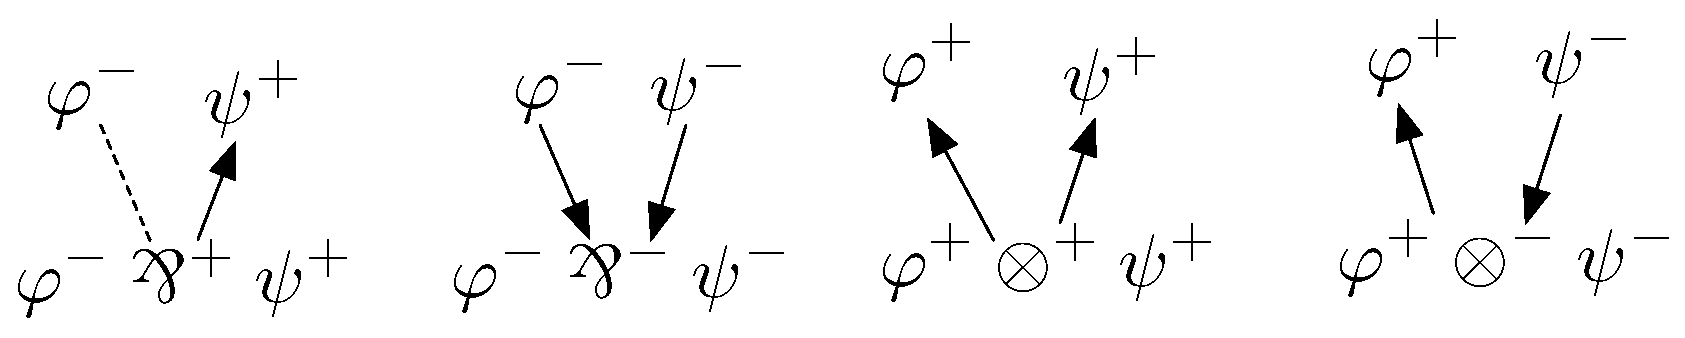
\includegraphics[scale=0.4]{rules-original.eps}
 \end{center}
For brevity, we sometimes write only the top connectives of labelling
formulae.
In that case, these branching nodes are denoted like this.
 \begin{center} %rules
  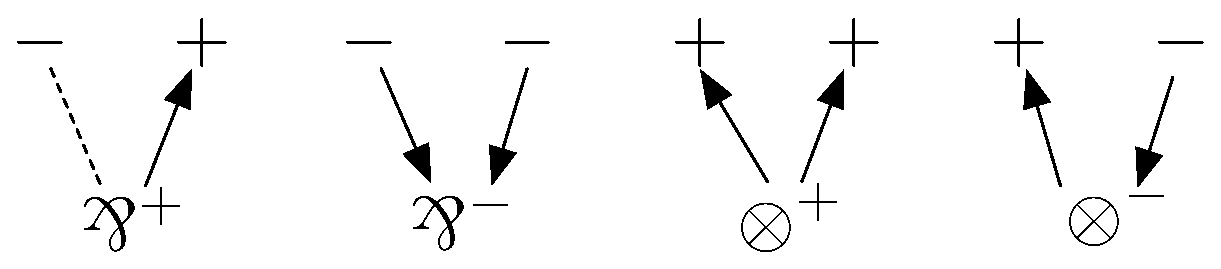
\includegraphics[scale=0.4]{rules.eps}
 \end{center}
We call arrows with upward (resp. downward) signs
\textit{up-edges}\index{up-edge}
(resp. \textit{down-edges}\index{down-edge}).
The dashed child of a $\parr^+$ node~$p$ is the node which the dashed
line from $p$ reaches.
The branching nodes labelled by $\parr^+, \parr^-, \otimes^+$ and
$\otimes^-$ are called \textit{operator nodes}.

When we add axiom edges, $\bot$-branches (shown below)
and some other operator nodes (shown above)
we obtain an
essential net of $\phi$.
Due to the arbitrarity of choosing axioms and $\bot-$-branches,
there are more than one essential nets for a formula%
\footnote{\citet{murawski2003} restricts the class of formulae to linearly balanced
formulae so that the essential net is uniquely determined.}.
 \begin{center}
  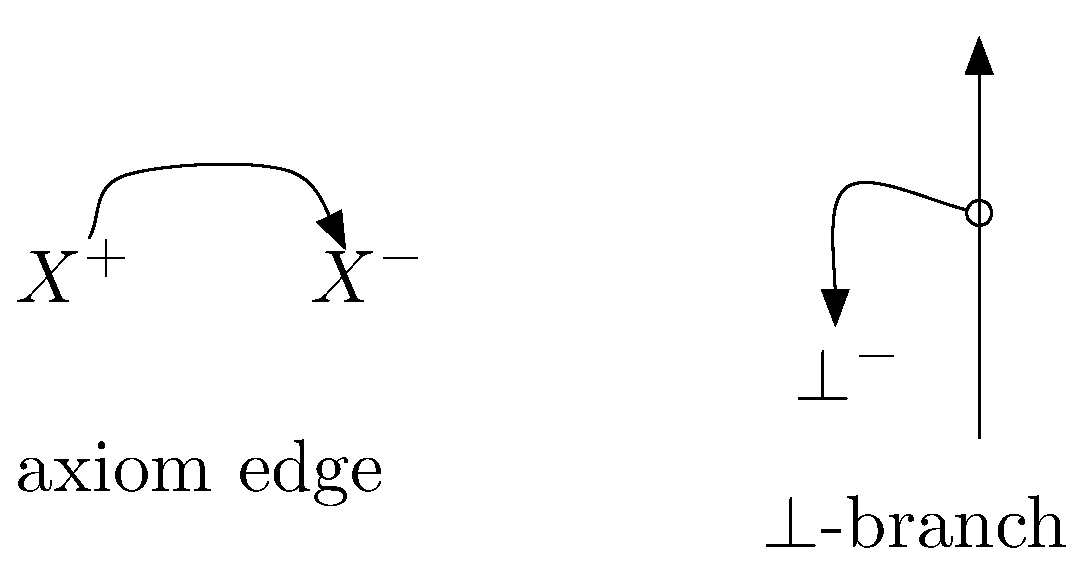
\includegraphics[scale=0.4]{axiom-cut.eps}
 \end{center}

 \begin{example}[An essential net of the Amida axiom] \label{essential-amida}
  Here is one of the essential nets of
  the Amida axiom $(X^-\parr^+Y^+)\otimes^+(Y^-\parr^+ Y^+)$.
   \begin{center}
    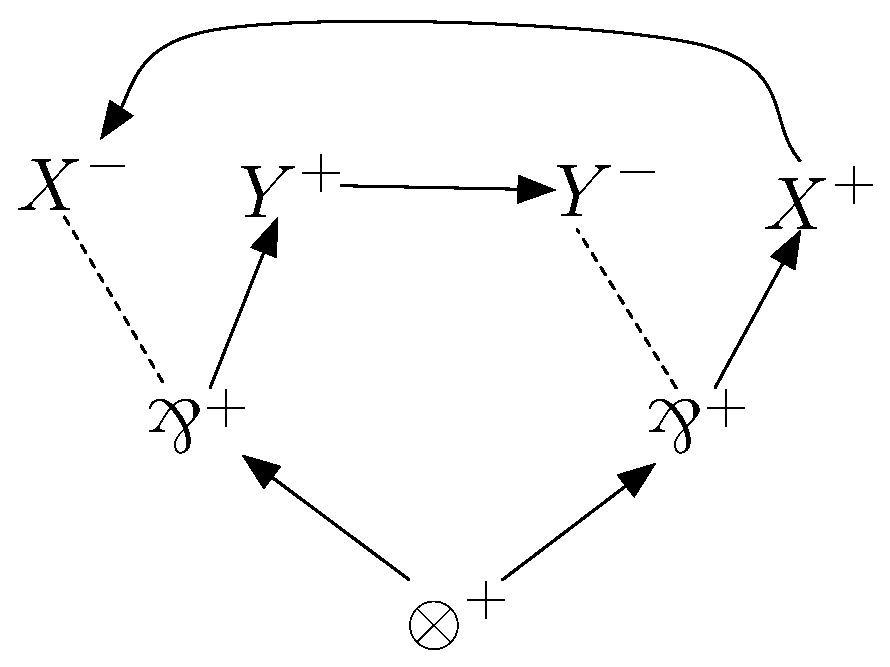
\includegraphics[scale=0.4]{amida-essential.eps}
   \end{center}
 \end{example}
 However, the essential net in \thref{essential-amida} is rejected by
 the following correctness criterion.
  \begin{definition}[Correct essential nets]
\begin{enumerate}
 \item Any leaf labelled with $X^+$ (resp. $Y^-$) is connected to a
       unique leaf labelled with $X^-$ (resp. $Y^+$).
       Any leaf labelled with $\bot^-$ is connected to a $\bot$-branch
       ($\one^+$ does not have to be connected to anything).
 \item The directed graph formed by up-edge, down-edge, axiom edges and
       $\bot$-branches is acyclic.
 \item \label{conditionL}
       for every $\parr^+$-node~$p$, every path from the root that reaches
       $p$'s dashed child also passes through $p$.
\end{enumerate}
  \end{definition}
The essential net in Example~\ref{essential-amida} is not correct for
condition~\ref{conditionL}.  Actually, Amida axiom does not have
any correct essential net.

 \begin{theorem}[Esseential nets for
  IMLL by~\citet{lamarche2008,murawski2003}]
  \label{essential-ok}
  An IMLL formula~$\phi$ is provable in IMLL iff there exists a correct essential net
  of $\phi$.
 \end{theorem}
 \begin{proof}
  \citet{lamarche2008} uses a common technique of decomposing an
  essential net from the bottom.
  \citet{murawski2003} chose to reduce the problem to sequents of special forms
  called regular.
 \end{proof}

 Actually, Lamarche also considers the cut rule\footnote{As well as
 additive operators and exponentials.} in essential nets, thus
 we can include the following general axioms (as macros) and cuts (as
 primitives) and still use \thref{essential-ok}:
 \begin{center}
  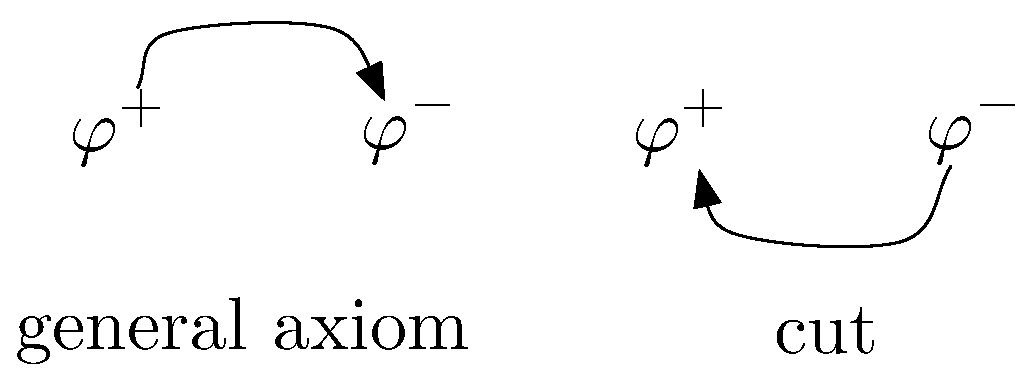
\includegraphics[scale=0.4]{general-axiom-cut.eps}\enspace.
 \end{center}

\subsection{Amida Nets}

 \begin{definition}[Amida nets]
  \label{def:amidanets}
For a hypersequent~$\hyper$,
\textit{Amida nets}\index{Amida nets} of $\hyper$ are inductively
  defined as
\begin{itemize}
 \item an essential net of $\hyper$ is an Amida net of $\hyper$
 \item for an Amida net of $\hyper$ with two different up-edges,
	\begin{center}
	 % twoedges
	 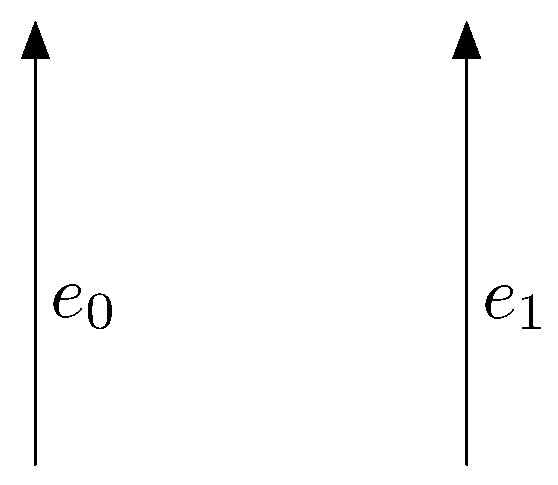
\includegraphics[scale=0.4]{twoedges.eps}
	\end{center}
       replacing these with
	\begin{center}
	 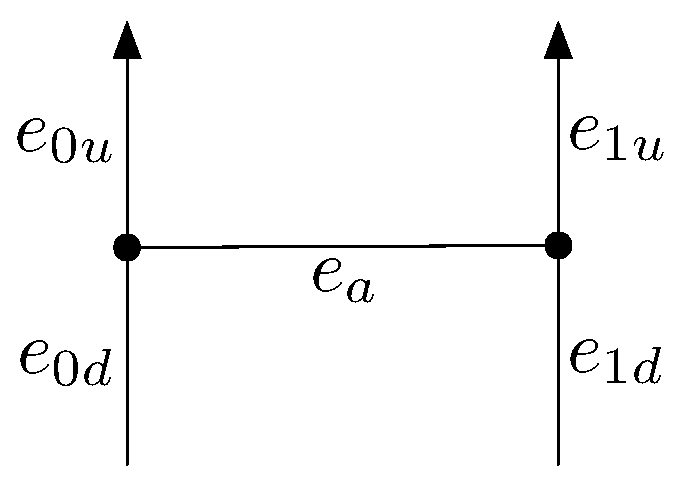
\includegraphics[scale=0.4]{twoedges_amida.eps}
	\end{center}
       yields an Amida net of $\hyper$,
       where the above component has two paths $e_{0d} e_a e_{1u}$
       and $e_{1d} e_a e_{0u}$.
 \item for an Amida net of $\hyper$ with a up-edge,
	\begin{center}
	 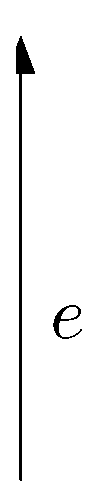
\includegraphics[scale=0.4]{oneedge.eps}
	\end{center}
       replacing this with
	\begin{center}
	 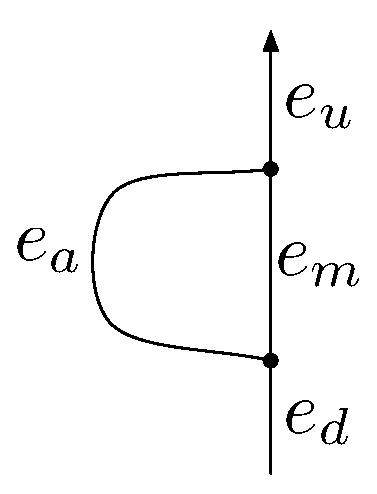
\includegraphics[scale=0.4]{oneedge_amida.eps}
	\end{center}
       yields an Amida net of $\hyper$,
       where the above component has
       one finite path $e_de_ae_u$
       and one infinite path $\cdots e_m e_a e_m e_a \cdots$.
\end{itemize}
 \end{definition}

 \begin{definition}[Correct Amida nets]
  A correct Amida net is an Amida net satisfying the three conditions
  of Definition~\ref{def:amidanets} where ``connected'' should be read
  ``connected by a path.''
 \end{definition}

 The Amida edge is not merely a crossing of vertical edges.
 See the difference between
 \begin{center}
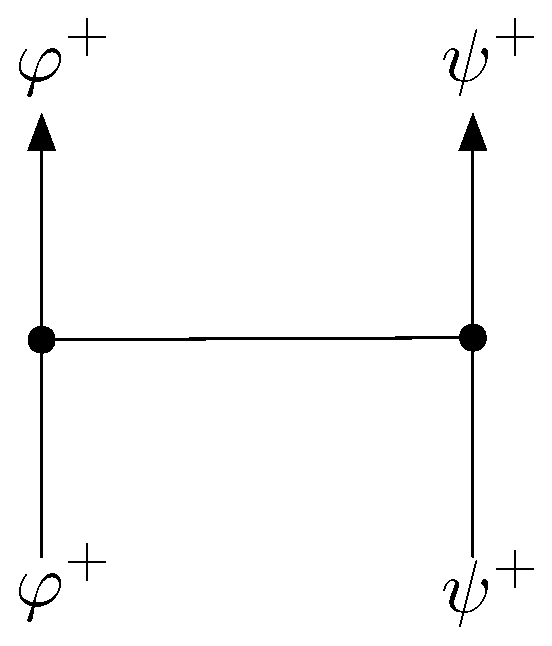
\includegraphics[scale=0.4]{twoedges_amida_without_label.eps}
 \end{center}
and
 \begin{center}

\includegraphics[scale=0.4]{crossing.eps}
 \end{center}
The difference is the labels at the bottom.
Although Amida edges cross the paths,
they do not transmit labels.
This difference causes Amida nets to validate Amida axiom.
 \begin{example}[Amida net for the Amida axiom]
  The Amida net for the Amida axiom $(X\limp Y)\otimes(Y\limp X)$.
   \begin{center}
    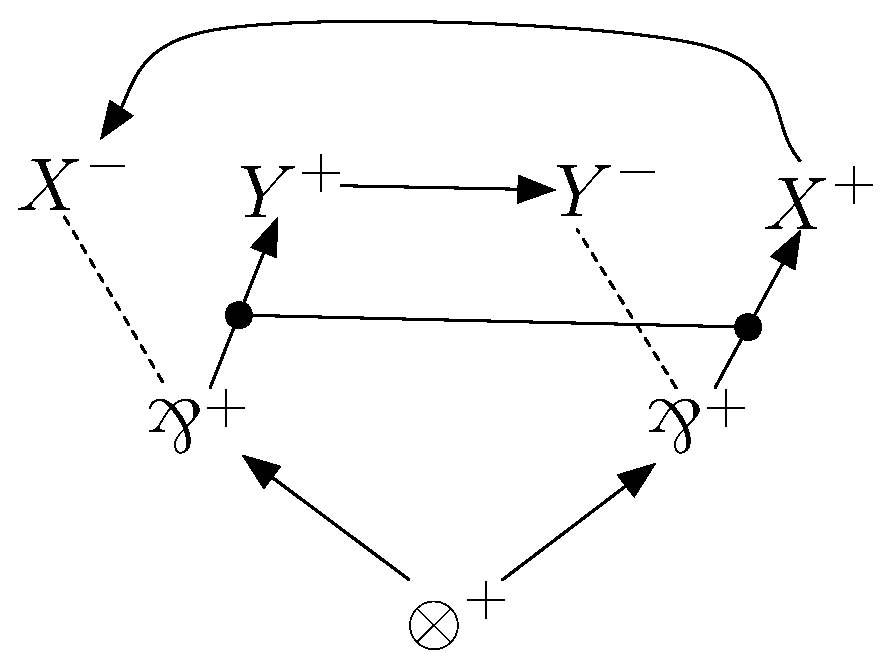
\includegraphics[scale=0.4]{amida-axiom.eps}
   \end{center}
  In terms of the set of paths, the above Amida net is equivalent to the
  following essential net for $(X\limp X)\otimes (Y\limp Y)$.
   \begin{center}
    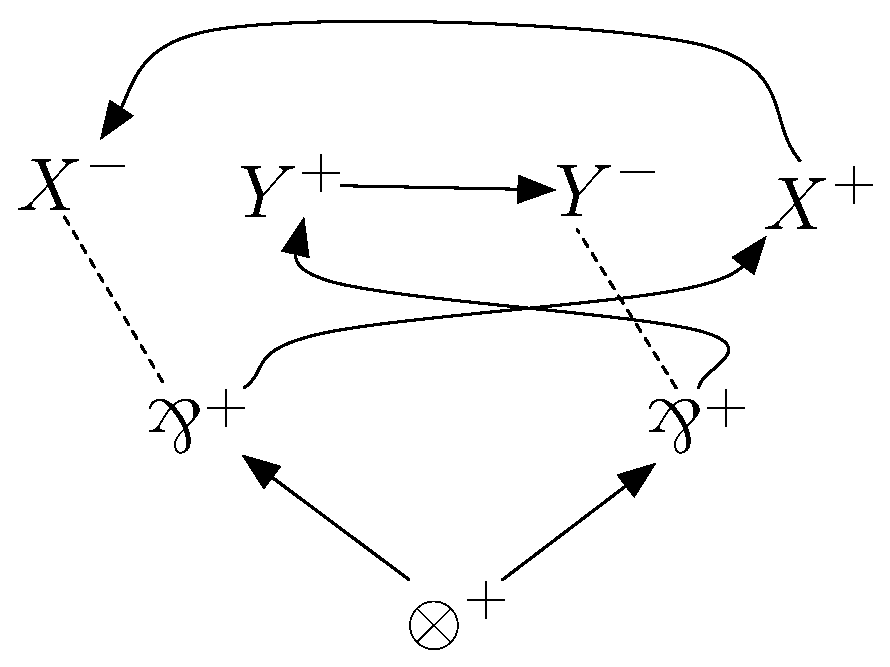
\includegraphics[scale=0.4]{amida-axiom-cross.eps}
   \end{center}
 \end{example}

\subsection{Soundness and Completeness of Amida nets}

 \begin{theorem}[Completeness of Amida nets]
  If a hypersequent $\hyper$ is derivable,
  there is a correct Amida net for $\hyper$.
 \end{theorem}
 \begin{proof}
  Inductively on hypersequent derivations.
  The Sync rule is translated into
   \begin{center}
    \fix{fill}
   \end{center}
 \end{proof}
 \begin{theorem}[Soundness of Amida nets]
  Inductively on the derivation of $\hyper$,
  we can translate a sequent calculus proof into a correct Amida net.
 \end{theorem}
 \begin{proof}
  From a correct Amida net, first we move the Amida edges upwards
  until they are just below axiom edges.

The translation moves are as follows.
 \begin{center}
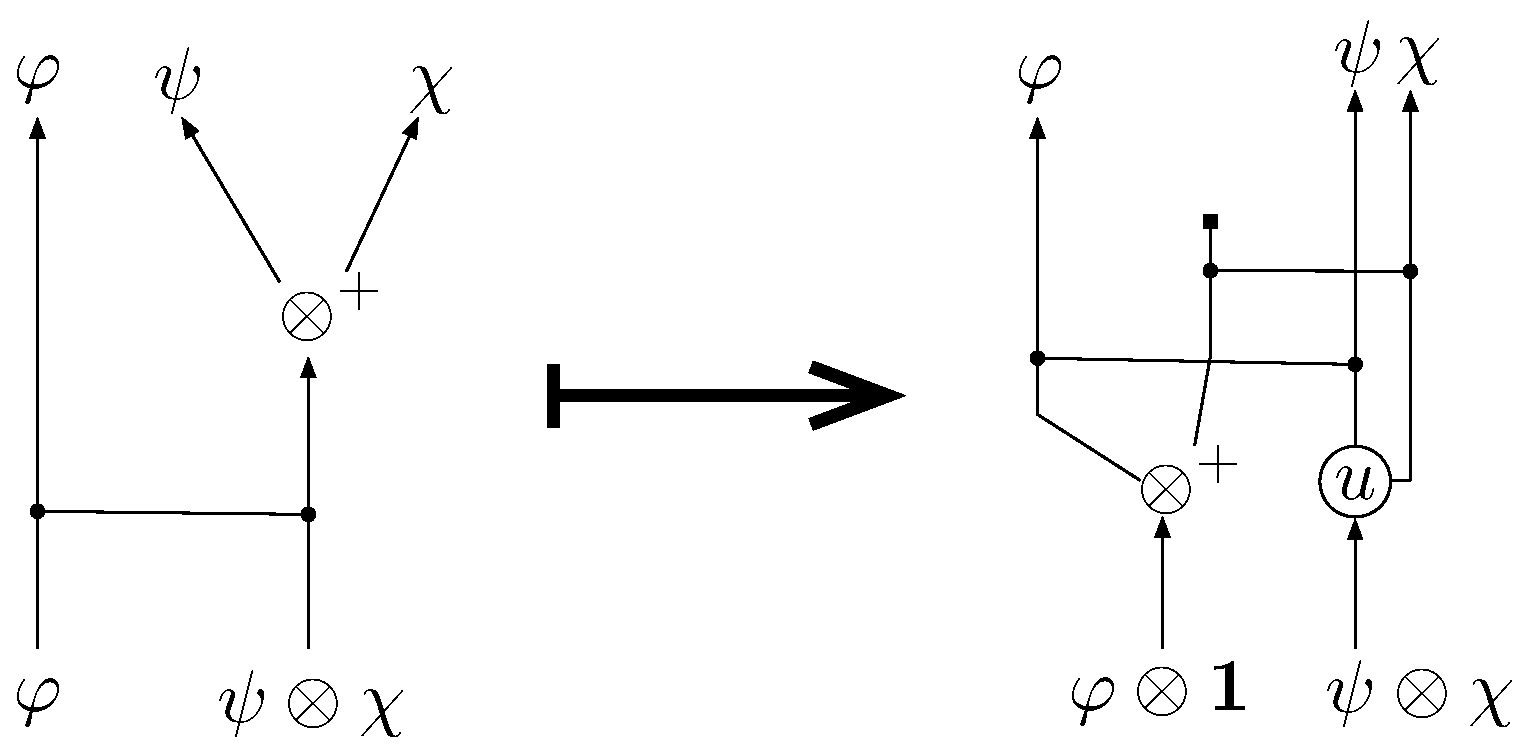
\includegraphics[scale=0.4]{tensor-move.eps}
\\
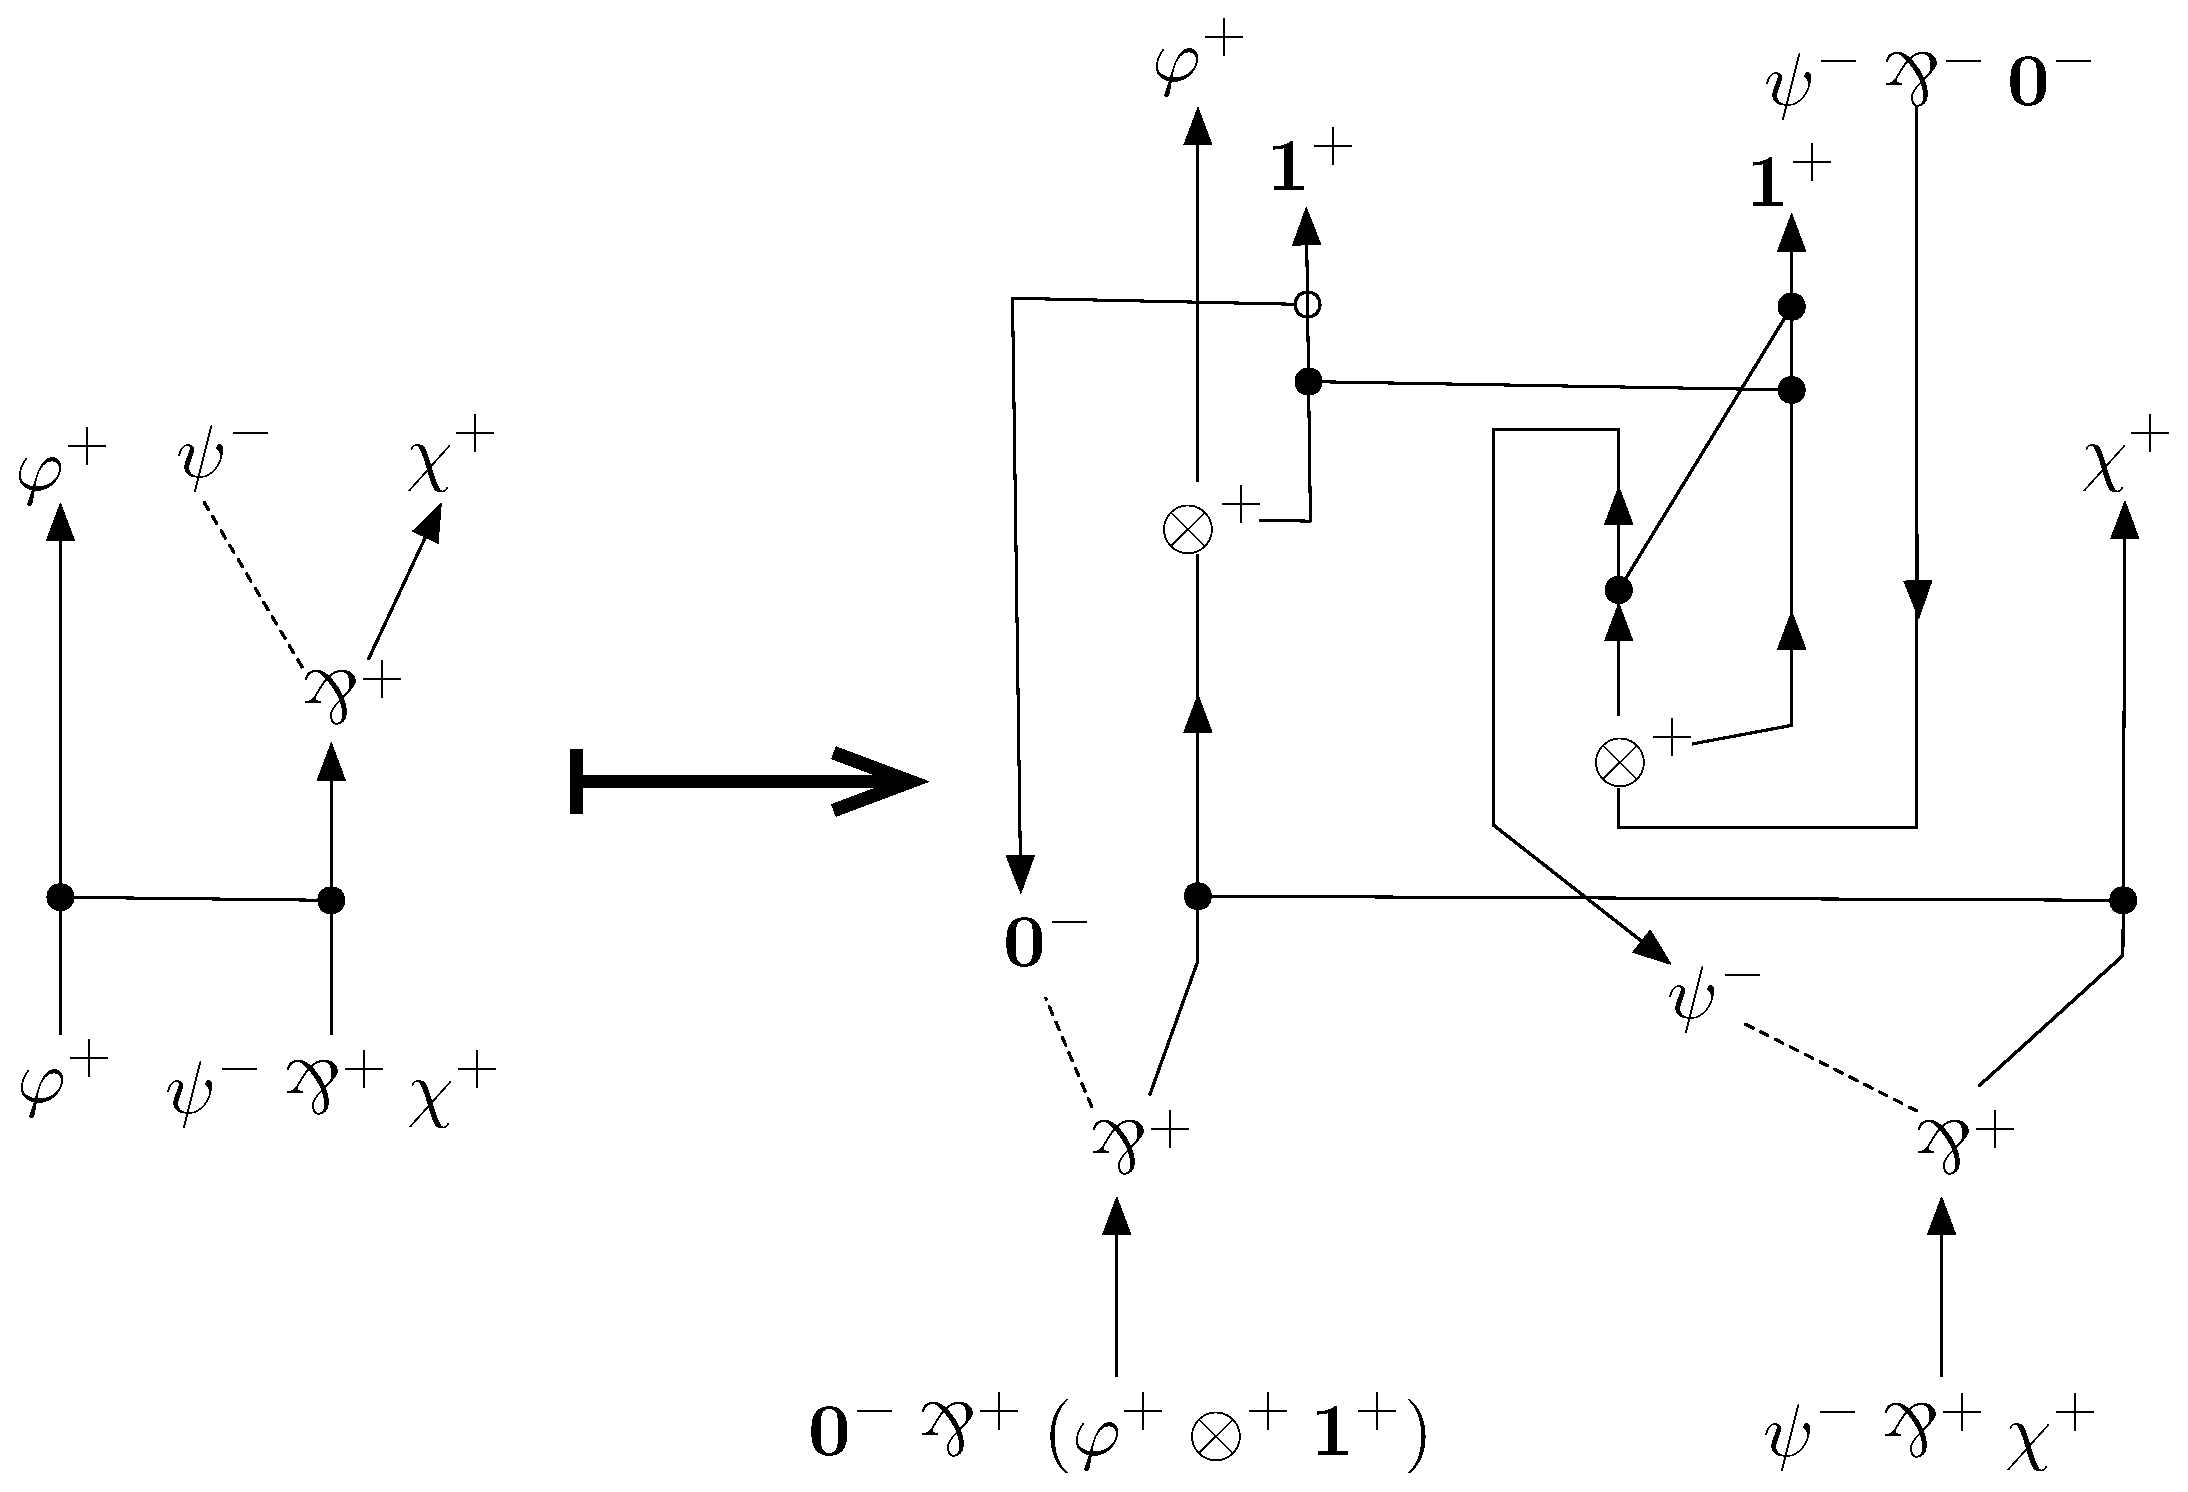
\includegraphics[scale=0.35]{parr-move.eps}
 \end{center}
These translations have two properties.
\begin{enumerate}
 \item When the original (substituted to a larger picture)
       is a correct Amida net, the translation (substituted to the same
       larger picture) is also a correct Amida net.
 \item The endpoints of the translation corresponds to the endpoints of
       the original, and the corresponding endpoints have the same label
       (up to logical equivalence in IMLL).  In case of $\otimes$
       translation, $\phi$ and
       $\phi\otimes \one$ are logically equivalent because $\one$ is the
       unit of $\otimes$.
       In case of $\parr$ translation, $\phi$ and $0\parr \phi$ are
       logically equivalent because $0$ is the unit of $\parr$.
\end{enumerate}
For checking the first condition, it is enough to follow the paths
(crossing all Amida edges).
For the second condition, it is enough to follow the vertical edges
except the Amida edges.

The $\otimes$ move introduces Amida edges only above the branching rules.
Although the $\parr$ move introduces an Amida edge below a
branching rule, that branching rule is of $\otimes$ nature.
Also, the $\parr$ move introduces an Amida edge below $\psi$-axiom link,
which is actually a macro.  So we have to continue applying the
translation moves in the macro.  However, Since $\psi$ is a strictly
smaller subformula of $\psi\parr\chi$, this does not cause infinite
recursion.

Then, by these translation moves,
the whole Amida net is decomposed vertically into three layers.
At the top, there is a layer with only Axiom edges.
In the middle, there is a layer with only vertical edges and Amida
edges.
At the bottom, there is a layer which contains only ordinary
essential net nodes.

Since the middle layer is an Amida lottery, it defines a permutation.
That permutation can be expressed as a product of transpositions, so
that
the original Amida lottery is equivalent to a loop-less Amida lottery.
A loop-less Amida lottery is an encoding of a hypersequent derivation
that consists of only Sync rules.

After we encode the top and the middle layer, encoding the bottom layer
is the same as \fix{Lamarche's theorem which}
 \end{proof}



We expect that it is possible to add Amida edges to
the full intuitionistic logic following
\citet{groote1999}
\fix{cite de groote / cite Lamarche}


\section{Related Work}

\subsection{Linear Logic and Session Types}

One promising approach is using session types~\citep{honda-session}.
Session types aims at typing channels and processes in $\pi$-calculus so
that the process execution is deterministic and not ending in deadlock.
In general session type systems are not based on well-known logic.



\subsubsection{Pfenning}

\citet{pfenning2010} provide a type system for a fragment of $\pi$-calculus.
Their type system imposes too strong a discipline
than necessary to provide deadlock freedom.
The escrowing process $P$ below is not typable in their type
system:
\[
 P = \sendterm x y{\recvterm x a {\recvterm y b {\sendterm x b
 {\sendterm y a 0}}}}\enspace.
\]
The process first emits a channel~$y$ through channel~$x$ and then
exchanges inputs from $x$ and $y$ into outputs to $y$ and $x$.
Following the informal description of types in \citep{pfenning2010},
the process~$P$ should be typable as
\[
 \vdash P::x:(A\limp B)\otimes(B\limp A)\enspace.
\]
However, such typing is not possible because $(A\limp B)\otimes (B\limp
A)$ is not a theorem of \fix{name} (DILL), the logic their type system
is based on.
In our type system, the following sequent is derivable
\begin{align*}
&
\tj{x}{\sendtype{(\sendtype{B}{\recvtype{A}\terminate})}{\recvtype B
{\sendtype A \terminate}}}
\tr\\
&\tj{
\nu(\tj{y}{\sendtype B{\recvtype A \terminate}}).
{\sendterm x{y_L}{\recvterm x a {\recvterm {y_R} b {\sendterm x b {\sendterm
{y_R} a {\ign{x,y}0}}}}}}
}{\one}
\end{align*}
The resulting sequent indicates that the process is typable with one
open channel~$x$ that emits
a channel to/from which one can send~$B$ and receive~$A$, receives a
value of $B$ and
sends a value of $A$.
This example shows that our type system is strictly more flexible than
the type system in \citet{pfenning2010}.
Moreover, we still ensure deadlock freedom in the sense that all typed
processes reduce to the canonical form~(\thref{convergence}).

The most complicated example in \citet{pfenning2010} is the following
one, which can be typed and evaluated in our framework as well.

 \begin{example}[Drink server example from \citet{pfenning2010} in Amida
  calculus]
  \begin{align*}
   ServerProto &= (N\limp I \limp (N\otimes \one))\with (N\limp( I
  \otimes \one)) \\
   &= (\sendtype N {\sendtype { I} {\recvtype N \terminate}}) \with
   (\sendtype N {\recvtype { I} \one})
  \end{align*}
  $N$ stands for the type of strings and $I$ stands for the type of
  integers, but following \citet{pfenning2010}, we identify both $N$ and
  $I$ with $\one$.
  Here is the prototype of the server, that serves one client and
  terminates.\\
  \[
   Serv = \lpair{\recvterm s {pn} {\recvterm s {cn} {\sendterm s {rc}
  {\ign {pn, cn, s} 0}}}
  ,\quad
  \recvterm s {pn} {\sendterm s {pr} {\ign{s,pn} 0}}
  }
  \]
  We can derive a sequent $\tj{s}{\overline{SP}}\tr\tj{Serv}\one$.
  \fix{how}

  Using this, we can also implement a server that can replicate itself
  and serve many clients.  Below, $SP$ abbreviates $ServerProto$.
  \begin{center}
   \AxiomC{$\tj{s}{\overline{SP}}\tr\tj {Serv}{\one}$}
   \AxiomC{}
   \UnaryInfC{$\tj{x}{SP}\tr\tj{x}{SP}$}
   \UnaryInfC{$\tj{z}\one,\tj{x}{SP}\tr\tj{\ign z x}{SP}$}
   \BinaryInfC{$\tj{s}{\overline{SP}},\tj{x}{SP}\tr\tj{\ign{Serv}x}{SP}$}
   \UnaryInfC{$\tr\tj{\nu(\tj{s}{SP}).\ign{Serv[s_R/s]}{s_L}}{SP}$}
   \UnaryInfC{$\tr\tj{\nu(\tj{s}{SP}).\ign{Serv[s_R/s]}{s_L}}{
   SP}$}
   \DisplayProof
  \end{center}


  Here is one client:
  \begin{center}
   \AxiomC{}
   \UnaryInfC{$\tr\tj{0}\one$}
   \UnaryInfC{$\tj{s}{\terminate}\tr\tj{\ign s 0}\one$}
   \UnaryInfC{$\tj{s}{\terminate},
   \tj{pr}{I}\tr\tj{\ign{pr,s} 0}\one$}
   \UnaryInfC{
   $ \tj{s}{\recvtype {I} {\terminate}} \tr\tj{
   \recvterm s {pr} {\ign{pr,s} 0}
   }{\one}$
   }
   \AxiomC{}
   \UnaryInfC{$ \tr\tj{tea}{N} $}
   \BinaryInfC{
   $ \tj{s}{\sendtype N {\recvtype {I} \terminate}} \tr\tj{
   \sendterm s {tea}
   {\recvterm s {pr} {\ign{pr,s} 0}}
   }{\one}$
   }
   \UnaryInfC{
   $ \tj{s}{ServerProto} \tr\tj{
   \letin s {\lpair{\_, s}} {
   \sendterm s {tea}
   {\recvterm s {pr} {\ign{pr,s} 0}}}
   }{\one}$
   }
   \DisplayProof
  \end{center}
  We abbreviate the process as $QClnt_s$.
  In words, the client first chooses the server's second protocol, which
  is price quoting, and asks the price of the tea, receives the price
  and terminates.


  We can combine the server with two clients.
   \begin{center}
   \end{center}

  Here is an evaluation of the combined system of the server and the two
  clients.
 \end{example}

\subsubsection{Wadler}

\citet{wadler2012propositions} gave a type system for a process
calculus based on classical linear logic.
Although the setting is classical, the idea is more or less the same as
\citet{pfenning2010}.
Wadler's type system cannot type the escrowing process above.
Worse, \citet{wadler2012propositions} does not recognize this
\[
 \sendterm x y{\recvterm x a {\recvterm y b {\sendterm x b {\sendterm y
 a 0}}}}
\]
as a process at all.
His grammar requires the output construction to be used in the form
\[
 \sendterm x y {(P\mid Q)}
\]
where $x$ is bound in $Q$ but not in $P$ and $y$ is bound in $P$ but not
in $Q$.
Of course, there is a way to escape the above restriction by making $P$
and $Q$ communicate, but that option is prohibited by the typing rules.

Wadler uses classical linear logic rather than intuitionistic linear
logic.
He justifies the choice for ``greater simplicity and symmetry.''
Adding Amida axiom to the classical linear logic is a future direction.
One looming difficulty is as follows.
In classical multiplicative linear logic,
adding Amida edges to proof nets seems harder than the intuitionistic case
because classical MLL proof nets have no direction on edges.
After a path crosses an Amida edge, the author has no idea which
direction the path should continue.

In other respects,
Wadler's type system is similar to ours;
our abbreviations are largely taken from Wadler's translations.

\subsubsection{Giunti and Vasconcelos}

\citet{giunti2010} gives a type system for the pi calculus, which is
extremely similar to our type system.
They say ``the goale of this work is to equip types with a contsructor
able to denote the two ends of a same
channel.''~\citep[Introduction]{giunti2010}
One of their typing rules
 \begin{center}
  \AxiomC{$\G,x\colon(S,\overline S)\tr P$}
  \UnaryInfC{$\G\tr(\nu x)P$}
  \DisplayProof
 \end{center}
 is similar to a rule in \thref{typing_connection}
 \begin{center}
  \AxiomC   {$\hypert\hmid
  \G,\tj{x}{\phi^\ell},\tj{y}{\overline{\phi^\ell}}\tr\tj t \psi$}
  \UnaryInfC{$\hypert\hmid
  \G\tr\tj{\nu\tj{x}{\phi^\ell}.t[x_L/x][x_R/y]}{\psi}$}
  \DisplayProof\enspace.
 \end{center}
 Usually, the Curry--Howard correspondence is followed from logical world
 to the programming world: for an alraedy known logic, a new lambda
 calculus is invented (e.g.~\fix{lambda mu kakutani kimura pfenning alex
 sympson so on}).  However, in our case, it seems that we have just
 found a logic called Amida logic that corresponds to an already known
 typing descipline invented by \citet{giunti2010}.
 It will be worthwhile to compare their system with our type system.

 \subsubsection{Double Binder}
 Our $\nu x$ notation binds two variables $x_L$ and $x_R$.
 This is similar to the double binder $\nu x_L x_R$ appearing in
 \citet{gay2010}.

 \subsection{Join calculus}
\fix{mention join calculus here or in related work}

\subsection{Delimited Continuation}
\fix{fill}

 \subsection{Logic Programming}

 There are at least two ways to interpret logics computationally.
 One is proof reduction, which is represented by $\lambda$-calculi.
 The other is proof searching.  What is the meaning of Amida axiom in
 the proof searching approach?

 Let us cite an example from \citet[A.2]{kobayashi-yonezawa}:
 \begin{quote}
  Consumption of a message $m$ by a process $m\limp B$ is represented by
  the following deduction:
  \[
   (m\otimes(m\limp B)\otimes C)\limp (B\otimes C)
  \]
  where $C$ can be considered as other processes and messages, or an environment.
 \end{quote}
 In existence of Amida axiom,
 the inverse
 \[
  (B\otimes C)\limp (m\otimes (m\limp B))\otimes C
 \]
 is derivable.
 This suggests that the Amida axiom states that some
 computation is reversible.  We are not sure whether this is very
 useful within the realm of reversible computation~\citep{revcon}.

\section{Discussion}

\subsection{Categorical Considerations}
One might want to ask whether we can model the logic with
a symmetric monoidal closed category~\citep{blute2004category}
  with identified isomorphisms
$\sigma_{ABCD}\colon (A\limp B)\otimes (C\limp D)\rightarrow (A\limp D) \otimes
 (C\limp B)$, with naturality conditions.
 Before considering equality among morphisms,
 we know there is a non-trivial example.
  \begin{example}[A symmetric monoidal closed category with swaps]
   \label{smcc}
   The preorder formed by objects as integers and morphisms as the usual
   order among integers~$\le$
   forms a symmetric monoidal closed category with swaps
   when we interpret $\otimes$ as addition and
   $m \limp n$ as $n-m$.
  \end{example}
  On the other hand,
  if we take another formulation requiring natural isomorphisms
  $\mathcal C(C,A)\times\mathcal C(D,B) \cong \mathcal C(D,A)\times
  \mathcal C{(C,B)}$,
  only singletons can be preorder models because $\tuple{id_A,id_B}$ is
  mapped to $\tuple{f,g}$ where $f\colon A\rightarrow B$ and $g\colon
  B\rightarrow A$ for any two objects $A$ and $B$.

A straightforward reading of evaluation rules gives somewhat complicated
equality conditions for morphisms.
The condition says the following diagram commutes:
\[
   \begin{CD}
    (A\limp B)\otimes (C\limp D) @>{d_{ABCD}}>> (A\otimes C)\limp(B\otimes D)\\
    @VV{\sigma_{ABCD}}V @VV{id\limp s_{B,D}}V\\
    (A\limp D)\otimes (C\limp B) @>{d_{ADCB}}>> (A\otimes C)\limp (D\otimes B)
   \end{CD}
\]
where $d_{ABCD}$ is induced by adjunction between $\otimes$ and $\limp$
 from a morphism
 $((A\limp B)\otimes (C\limp D))\otimes (A\otimes C)\rightarrow
 (B\otimes D)$, which is provided by symmetric monoidal closed
 properties.

\subsection{Multiparty, recursions, \ldots}
Our type system has a drawback of having only finitely many processes.
We expect it straightforward to overcome this weak point by
add recursions in our type system.
As a guidance we can take $\mu$MALL of \citet{mumall}.

Our operational semantics is different from the standard session
calculus.  Since our operational semantics seems more liberal,
if we limit it, we do not lose type safety.  However, if we do not
choose a suitable class of reductions, the reduction can be
nondeterministic.
The reconcilation of lienarity and pi-calculus style operational
semantics has already been considered by
\citet{kobayashi-pierce-turner} so we expect their work to be a
guidance toward finding a more traditional operational semantics.

It is tempting to add modalities showing agents to types so that the
modalities show agents and then study the relationship with the
multiparty session types~\citep{sync-multi-session, async-multi-session}.
For that, intuitionistic epistemic logic~\citet{hirailpar,hiraimaster}
will be useful.

In order to implement this lambda calculus, we need linear types.
The uniqueness type of Clean~\fix{cite} is not enough because
their type system allows weakening.

\fix{compare with linear ML}

\section{Conclusion}

We found Amida logic, which can be characterized by Amida axiom
$(\phi\limp\psi)\otimes(\psi\limp\phi)$ on top of IMALL.
The logic has an application for encoding process calculi and session type
system.
As a technique, we first used conjunctive hypersequents,
where components in a hypersequent are interpreted conjunctively rather
than disjunctively.